% -*- coding: utf-8; -*-
% vim: set fileencoding=utf-8 :

% TODO BEFORE SUBMISSION
% be consistent between "IDs" and "ids" [SK prefers "IDs" to avoid it being read as a word]
% even more so between "ID" and "id" [NB: "id" is a word in English]
% \usepackage[sort]{natbib} or otherwise manually fix cites to be in ascending order
% redo fig 5 to have better resolution

% TODO BEFORE FINAL
% - uncomment acks

% The paper on using Luau telemetry to measure the effectiveness of type error reporting.

\documentclass[english,submission,cleveref]{programming}
%% use 'submission' for initial submission, remove it for camera-ready (see 5.1)

\usepackage{todonotes}

%%\overfullrule=1mm

%% BEGIN tobias pape 2021-11-06
% Why do we need this? To have headings in the abstract.
\makeatletter
\newcommand*\abstractpart[1]{\unskip\par\noindent{\firamedium\color{P@GrayFG}{#1}}\enspace}
\makeatother
%% END

\usepackage{alltt}
% Not sure why <Programming> is recommending non-standard tools
% \usepackage[backend=biber]{biblatex}
\usepackage[export]{adjustbox}
\usepackage{amssymb}
\usepackage{calc}
\usepackage{colortbl}
\usepackage{listings}
\usepackage{mathpartir}
\usepackage{pifont}
% Errors with
% ! Undefined control sequence.
% <argument> \l__siunitx_number_implicit_plus_bool 
% l.61 \begin{document}
% using Mac TeXlive 20230313_2
% \usepackage{siunitx}
\usepackage{tikz}
\usepackage{subcaption}
\usepackage{wasysym}
\usepackage{xcolor}
\usetikzlibrary{shapes.geometric}

%%%%%%%%%%%%%%%%%%
\paperdetails{
  %% perspective options are: art, sciencetheoretical, scienceempirical, engineering.
  %% Choose exactly the one that best describes this work. (see 2.1)
  perspective=scienceempirical,
  %% State one or more areas, separated by a comma. (see 2.2)
  %% Please see list of areas in http://programming-journal.org/cfp/
  %% The list is open-ended, so use other areas if yours is/are not listed.
  area={Data mining for programming, Telemetry},
  %% You may choose the license for your paper (see 3.)
  %% License options include: cc-by (default), cc-by-nc
  % license=cc-by,
}
%%%%%%%%%%%%%%%%%%

%%%%%%%%%%%%%%%%%%
%% These data are provided by the editors. May be left out on submission.
%\paperdetails{
%  submitted=2023-1-31,
%  published=2016-10-11,
%  year=2016,
%  volume=1,
%  issue=1,
%  articlenumber=1,
%}
%%%%%%%%%%%%%%%%%%

\begin{document}

\title{Type Error Telemetry at Scale}
% lean, lite, modest, non-intrusive, private, ...
% {Millions of Type Errors} = 72M forced strict, 1/2M type error is disappointing!
%% \subtitle{Impersonal Telemetry to Measure User Experience}

%\titlerunning{DRAFT do not distribute}

% Alphabetical order for authors?

\author[a,b]{Ben Greenman}
\authorinfo{(\email{benjamin.l.greenman@gmail.com}) was a CIFellows 2020
postdoc at Brown Univesity and is now an assistant professor
at the recently-named Kahlert School of Computing at the University of Utah.}
\affiliation[a]{Brown University, Providence, RI, USA}
\affiliation[b]{University of Utah, Salt Lake City, UT, USA}
% \orcid{0000-0001-7078-9287}

\author[c]{Alan Jeffrey}
\authorinfo{(\email{ajeffrey@roblox.com}) is a Principal Software Engineer at Roblox.}
% \orcid{0000-0001-6342-0318}
\affiliation[c]{Roblox, San Mateo, CA, USA}

\author[a]{Shriram Krishnamurthi}
% \orcid{0000-0001-5184-1975}
\authorinfo{(\email{shriram@brown.edu}) is the Vice President of Programming Languages (no, not really) at Brown University.}

\author[c]{Mitesh Shah}
\authorinfo{(\email{mshah@roblox.com}) is Senior Engineering Director, Programmability, at Roblox.}

%\renewcommand{\shortauthors}{...}

%\authorrunning{DRAFT do not distribute}

\newcommand{\code}[1]{\texttt{#1}}
\newcommand{\FILL}{\textbf{FILL}}
\newcommand{\dotscale}[1]{\scalebox{0.72}{#1}}
\newcommand{\wideas}[2]{\makebox[\widthof{#2}][l]{#1}}
\newcommand{\twoline}[2]{\parbox[s]{1.4cm}{\flushleft#1\newline#2}}
\newcommand{\chkYes}{\dotscale{\CIRCLE}}
\newcommand{\chkMaybe}{\wideas{\dotscale{\Circle}}{\chkYes}}
\newcommand{\chkNo}{\wideas{}{\chkYes}}
\newcommand{\pct}[1]{\SI{#1}{\percent}}
\newcommand{\percentile}[1]{{#1}th~percentile}
\newcommand{\ptile}[1]{\textsc{p}{#1}}
\newcommand{\modefont}[1]{\texttt{#1}}
\newcommand{\mnocheck}{\modefont{nocheck}}
\newcommand{\mnonstrict}{\modefont{nonstrict}}
\newcommand{\mstrict}{\modefont{strict}}
\newcommand{\FS}{background}
\newcommand{\zerowidth}[1]{\makebox[0pt][l]{#1}}
\newcommand{\zeroheight}[1]{\raisebox{0pt}[0pt][0pt]{\(#1\)}}
\newcommand{\nK}[1]{#1\textsc{k}}
\newcommand{\stddev}[1]{\nK{#1}}
\newcommand{\gcell}[1]{\cellcolor{green!20}#1}
\newcommand{\ycell}[1]{\cellcolor{yellow!18}#1}
\newcommand{\ocell}[1]{\cellcolor{orange!29}#1}
\newcommand{\rcell}[1]{\cellcolor{red!30}$\!\!$#1$\!\!$}
\newcommand{\gbox}[1]{\colorbox{green!20}{#1}}
\newcommand{\ybox}[1]{\colorbox{yellow!18}{#1}}
\newcommand{\obox}[1]{\colorbox{orange!29}{#1}}
\newcommand{\rbox}[1]{\colorbox{red!30}{#1}}
\newcommand{\tefsfont}[1]{\textsc{#1}}
\newcommand{\tekey}{\tefsfont{te}}
\newcommand{\fskey}{\tefsfont{bg}}
\newcommand{\QALAN}{\FILL{} Alan:}
\newcommand{\panon}{pseudonymized}
\newcommand{\symbox}[1]{{\makebox[0.8em][c]{{#1}}}}
\newcommand{\addsym}{\symbox{\(\uparrow\)}}
\newcommand{\keepsym}{\symbox{\(=\)}}
\newcommand{\dropsym}{\symbox{\(\downarrow\)}}
% \newcommand{\dsymbox}[1]{\makebox[0.8em][c]{#1}}
% \newcommand{\dropsym}{\dsymbox{\raisebox{0ex}[0.9em]{\raisebox{0.5ex}{\vrule width 0.6em height 0.6pt}}}}

%%
%% The code below is generated by the tool at http://dl.acm.org/ccs.cfm.
%% Please copy and paste the code instead of the example below.

\begin{CCSXML}
<ccs2012>
<concept>
<concept_id>10002944.10011123.10010916</concept_id>
<concept_desc>General and reference~Measurement</concept_desc>
<concept_significance>500</concept_significance>
</concept>
</ccs2012>
\end{CCSXML}

\ccsdesc[500]{General and reference~Measurement}

\keywords{types, gradual typing, telemetry, user study, large-scale study}

\maketitle

\begin{abstract}
  \let\paragraph\abstractpart

  \paragraph{Context}
  %% What is the broad context of the work? What is
  %% the importance of the general research area?
  {Roblox Studio} lets millions of creators
  build interactive experiences by programming in a variant
  of Lua called Luau.
  The creators form a broad group, ranging from novices writing
  their first script to professional developers; thus, Luau
  must support a wide audience.
  As part of its efforts to support all kinds programmers, Luau includes an
  optional, gradual type system and goes to great lengths to minimize false
  positive errors.

  \paragraph{Inquiry}
  %% What problem or question does the paper
  %% address? How has this problem or question been
  %% addressed by others (if at all)?
  Since Luau is currently being used by many creators, we want to collect their feedback
  to improve the language and, in particular, the type system.
  The standard way to collect feedback at a large scale from creators working on
  real projects is to deploy client-side telemetry; however, we cannot
  scrape personal data or proprietary information, which means we cannot
  collect source code fragments, error messages, or even filepaths.
  The research questions are thus about how to conduct telemetry that
  is not invasive and obtain insights from it about type errors.

  \paragraph{Approach}
  %% What was done that unveiled new knowledge?
  We designed and implemented a pseudonymized, randomized telemetry system for Luau.
  Telemetry records include a timestamp, a session id, a reason for sending,
  and a numeric summary of the most recent type analyses.
  This information lets us study type errors over time
  without revealing private data.
  We deployed the system in Roblox Studio during Spring 2023
  and collected over 1.5 million telemetry records from over 340,000 sessions.

  \paragraph{Knowledge}
  %% What new facts were uncovered? If the
  %% research was not results oriented, what new
  %% capabilities are enabled by the work?
  We present several findings about Luau, all of which suggest that telemetry
  is an effective way to study type error pragmatics.
  One of the less-surprising findings is that opt-in gradual types are unpopular:
  there is an 100x gap between the number of untyped Luau sessions and the number
  of typed ones.
  One surprise is that the strict mode for type analysis is overly conservative
  about interactions with data assets.
  % Instead of using the flexible dynamic type, it uses a top type and requires
  % creators to down-cast assets.
  A reassuring finding is that type analysis rarely hits its internal limits on
  problem size.

  \paragraph{Grounding}
  %% What argument, feasibility proof, artifacts,
  %% or results and evaluation support this work?
  Our findings are supported by a dataset
  of over 1.5 million telemetry records.
  The data and scripts for analyzing it will be available in an artifact.

  \paragraph{Importance}
  %% Why does this work matter?
  Beyond the immediate benefits to Luau,
  our findings about types and type errors have implications
  for adoption and ergonomics in other gradual languages
  such as TypeScript, Elixir, and Typed Racket.
  Our telemetry design is of broad interest, as it reports on
  type errors without revealing sensitive information.

\end{abstract}


\section{Introduction}
\label{s:introduction}

{Roblox} is a platform for {shared virtual experiences} (typically 3D games), with
65~million Daily Active Users, and 14~billion hours of engagement in
April--June 2023~\cite{corp.roblox.com}.
There are over 5~million distinct user-created programs available on the platform thanks to a
worldwide community of 3~million creators.
Many of the creators program for fun or learning and may
not consider themselves software developers; others are professional
developers.

Creators program using the
{Luau} programming language~\cite{luau-lang.org},
an extension of {Lua~5.1~\cite{lua}}.
The main addition in Luau is a static type system that infers
types for all Luau programs on the fly, as creators modify the code.
These types are used primarily in IDE tooling such as autocomplete and
in API documentation~\cite{luau-autocomplete}, and indeed, creators
may be unaware that a typechecker is analyzing their code.
However, creators can opt in to receiving type error reports and they can write
their own types to guide designs and document their intentions.

Due to the broad community of creators, the goals of the Luau type
system are rather unique~\cite{bfj-hatra-2021}.
Whereas a traditional type system focuses on compilation and memory
safety, Luau takes a lenient approach by default and lets creators
gradually~\cite{st-sfp-2006,tf-popl-2008} migrate to rigorous checks
one module at a time.
In this way, for example,
students in code camps may begin in the \mnocheck{} mode that reports only
syntax errors; hobbyists can use \mnonstrict{} mode to identify
would-be runtime errors; and developers who need to ensure software
quality can rely on \mstrict{} mode.
(No matter the mode, a {\FS{}} type analysis still drives the IDE tools.)
Luau's types aim to support untyped designs, in the spirit of migratory
typing~\cite{tfffgksst-snapl-2017}, so that creators can switch modes without
needing to restructure their code in major, potentially-breaking, ways.

In this paper, we investigate methods for measuring the effectiveness
of the {Luau} type system.
The goal is to collect feedback at a large scale, with thousands
of participants maintaining real codebases.
Consequently, the measurements cannot reveal \emph{any} information about
source code, as it may contain personal data, proprietary algorithms, novel
game designs, and so on.
In comparison to prior work~(\cref{s:related}), which
with few exceptions~(e.g.,\cite{hlzbr-ecoop-2021}) is small in scale
or collects source code, we performed a large-scale study using \panon{}
{telemetry}.

Our starting point is a telemetry framework that is built in
to {Roblox Studio} and currently measures the effectiveness of
creation features.
%% \QALAN: can we be more specific? what's an example ... API usage?
This system randomly determines which sessions should report telemetry, and,
for those sessions, reports telemetry records back with a summary of the
session.

In this work, we design telemetry that collects data on type errors without
exposing source code, source locations, or even error message text (which
may contain revealing information).
The telemetry counts the number and \emph{kind} of type errors at various
levels of granularity.
Furthermore it maintains a client-side approximation of the latest source-code
edits and uses that to identify type errors that overlap with this edit range.
Telemetry records are correlated by session, using a \panon{} session
identifier and a timestamp.

With this telemetry data, we investigate research questions about
the adoption and benefits of type analysis:
\begin{description}
  \item[RQ1.]
    How many sessions use type analysis?
    How often do projects contain modules with different
    analysis modes?
    How often do sessions turn analysis off?
  \item[RQ2.]
    For modules that use type analysis:
    which errors arise,
    how do sessions respond,
    and which errors tend to persist despite subsequent edits?
  \item[RQ3.]
    What impact does type analysis have on the number of \FS{}
    errors?
    For example, do \FS{} errors pile up in unanalyzed projects?
\end{description}

Beyond their immediate revelance to {Luau},
answers to these questions have broad implications for the design
of gradually-typed languages.
Luau represents a large-scale combination of ideas from
gradual typing~\cite{st-sfp-2006,tfffgksst-snapl-2017,bat-ecoop-2014},
success typing~\cite{lindahl2006practical},
and semantic subtyping~\cite{CF05:GentleIntroduction,Jef22:SemanticSubtyping}.
Lessons from this experience can inform future applications.

At a higher level, this paper is the first to use telemetry 
to study a type checker.
It thus represents a step toward data-driven language design,
informed by many users' actual practice.
Our data captures over 340,000 sessions
that occured between February and April 2023
and covers thousands of type analysis errors
and millions of \FS{} errors.
By contrast to typical qualitative methods such as surveys and interviews, it
is not restricted to users' \emph{perceptions} about their work and it is not
limited to a small number of users.


\paragraph{Contributions}
\begin{itemize}
  \item
    Design of a low-overhead telemetry system
    that reports on type errors without revealing source code.

  \item
    Lessons from many thousands of type errors about
    adoption, persistent errors, and creators' responses.

  \item
    An available dataset of over 1.5 million telemetry records
    and scripts to analyze them.
    \emph{We intend to submit these in an artifact.}

\end{itemize}


\section{Context: {Roblox} and {Luau}}
\label{s:context}

% https://create.roblox.com/docs/scripting/luau

%% Most users of {Roblox Studio} do not opt in to type error
%% reporting (\pct{90},~\cref{s:data}), and so they do not see the ``squiggly underlining'' that
%% indicates a type error site. Nonetheless, the type inference system
%% still runs in the background (since it drives autocomplete and other
%% type-based tools), letting us see which type errors would have
%% been reported and whether users fix these errors over time.

{Roblox Studio} is a workbench that
combines {3D creation} tools and an Integrated
Developer Environment (IDE), as seen in \cref{fig:roblox-studio}.
The IDE includes an optional \emph{Script Analysis} widget that
reports syntax errors, type errors, and problems identified by
lint tools. The main editor widget can also highlight
source locations in code where reported errors occur.


\paragraph{Type Analysis Modes, \FS{} Analysis}

Creators can opt in to detailed error reports and highlights by
choosing a \emph{type analysis mode} for each script they write:
\begin{itemize}
  \item \mnocheck{}: report only syntax errors (the default),
  \item \mnonstrict{}: report syntax errors and a subset of high confidence type errors, or
  \item \mstrict{}: report syntax errors and all type errors.
\end{itemize}
Each run of type analysis can report several errors.
There is no guarantee that creators read every error.
In fact, creators who close the Script Analysis widget
will see highlights in their code but no further details.

In addition to the main type analysis, Roblox Studio takes a second pass over
every codebase with a \emph{\FS{}} analysis to infer autocomplete suggestions
and drive other IDE tools.
To infer precise types,
the \FS{} analysis uses rigorous checks very similar to those of
\mstrict{} mode (but not identical: see \cref{s:strict-vs-forcedstrict})
no matter what mode the creator declared for the script.
(Internally to Roblox Studio, this analysis is called \emph{forced strict}
because it ignores the creator's choice and applies strong checks.)
When it fails to infer a type, \FS{} analysis defaults to the unknown gradual
type~\cite{st-sfp-2006}.
Creators cannot see the errors reported by \FS{} analysis.

As an example of \mnonstrict{} mode, the following program only reports one error:
\begin{verbatim}
  --!nonstrict
  local x = { p = 5, q = nil }
  if condition then x.q = 7 end
  local y = x.p + x.q --> OK
  local z = x.r           --> UnknownProperty: Key 'r' not found in table 'x'
\end{verbatim}
In \mstrict{} mode, it reports two errors:
\begin{verbatim}
  --!strict
  local x = { p = 5, q = nil }
  if condition then x.q = 7 end
  local y = x.p + x.q --> TypeMismatch: Type 'nil' could not be converted into 'number'
  local z = x.r           --> UnknownProperty: Key 'r' not found in table 'x'
\end{verbatim}
In cases like this, where it is undecidable whether there will be a run-time error,
\mstrict{} mode errs on the side of reporting an error, and \mnonstrict{} mode errs on
the side of suppressing the error.

Both modes report the \code{UnknownProperty} error because
misspellings of property names are common enough to report in both
\mstrict{} and \mnonstrict{} mode.
\mnocheck{} reports no error because the program is syntactically valid.
See~\cite{bfj-hatra-2021} for a more detailed discussion of the rationale
behind the type systems.

\begin{figure}[t]\centering
  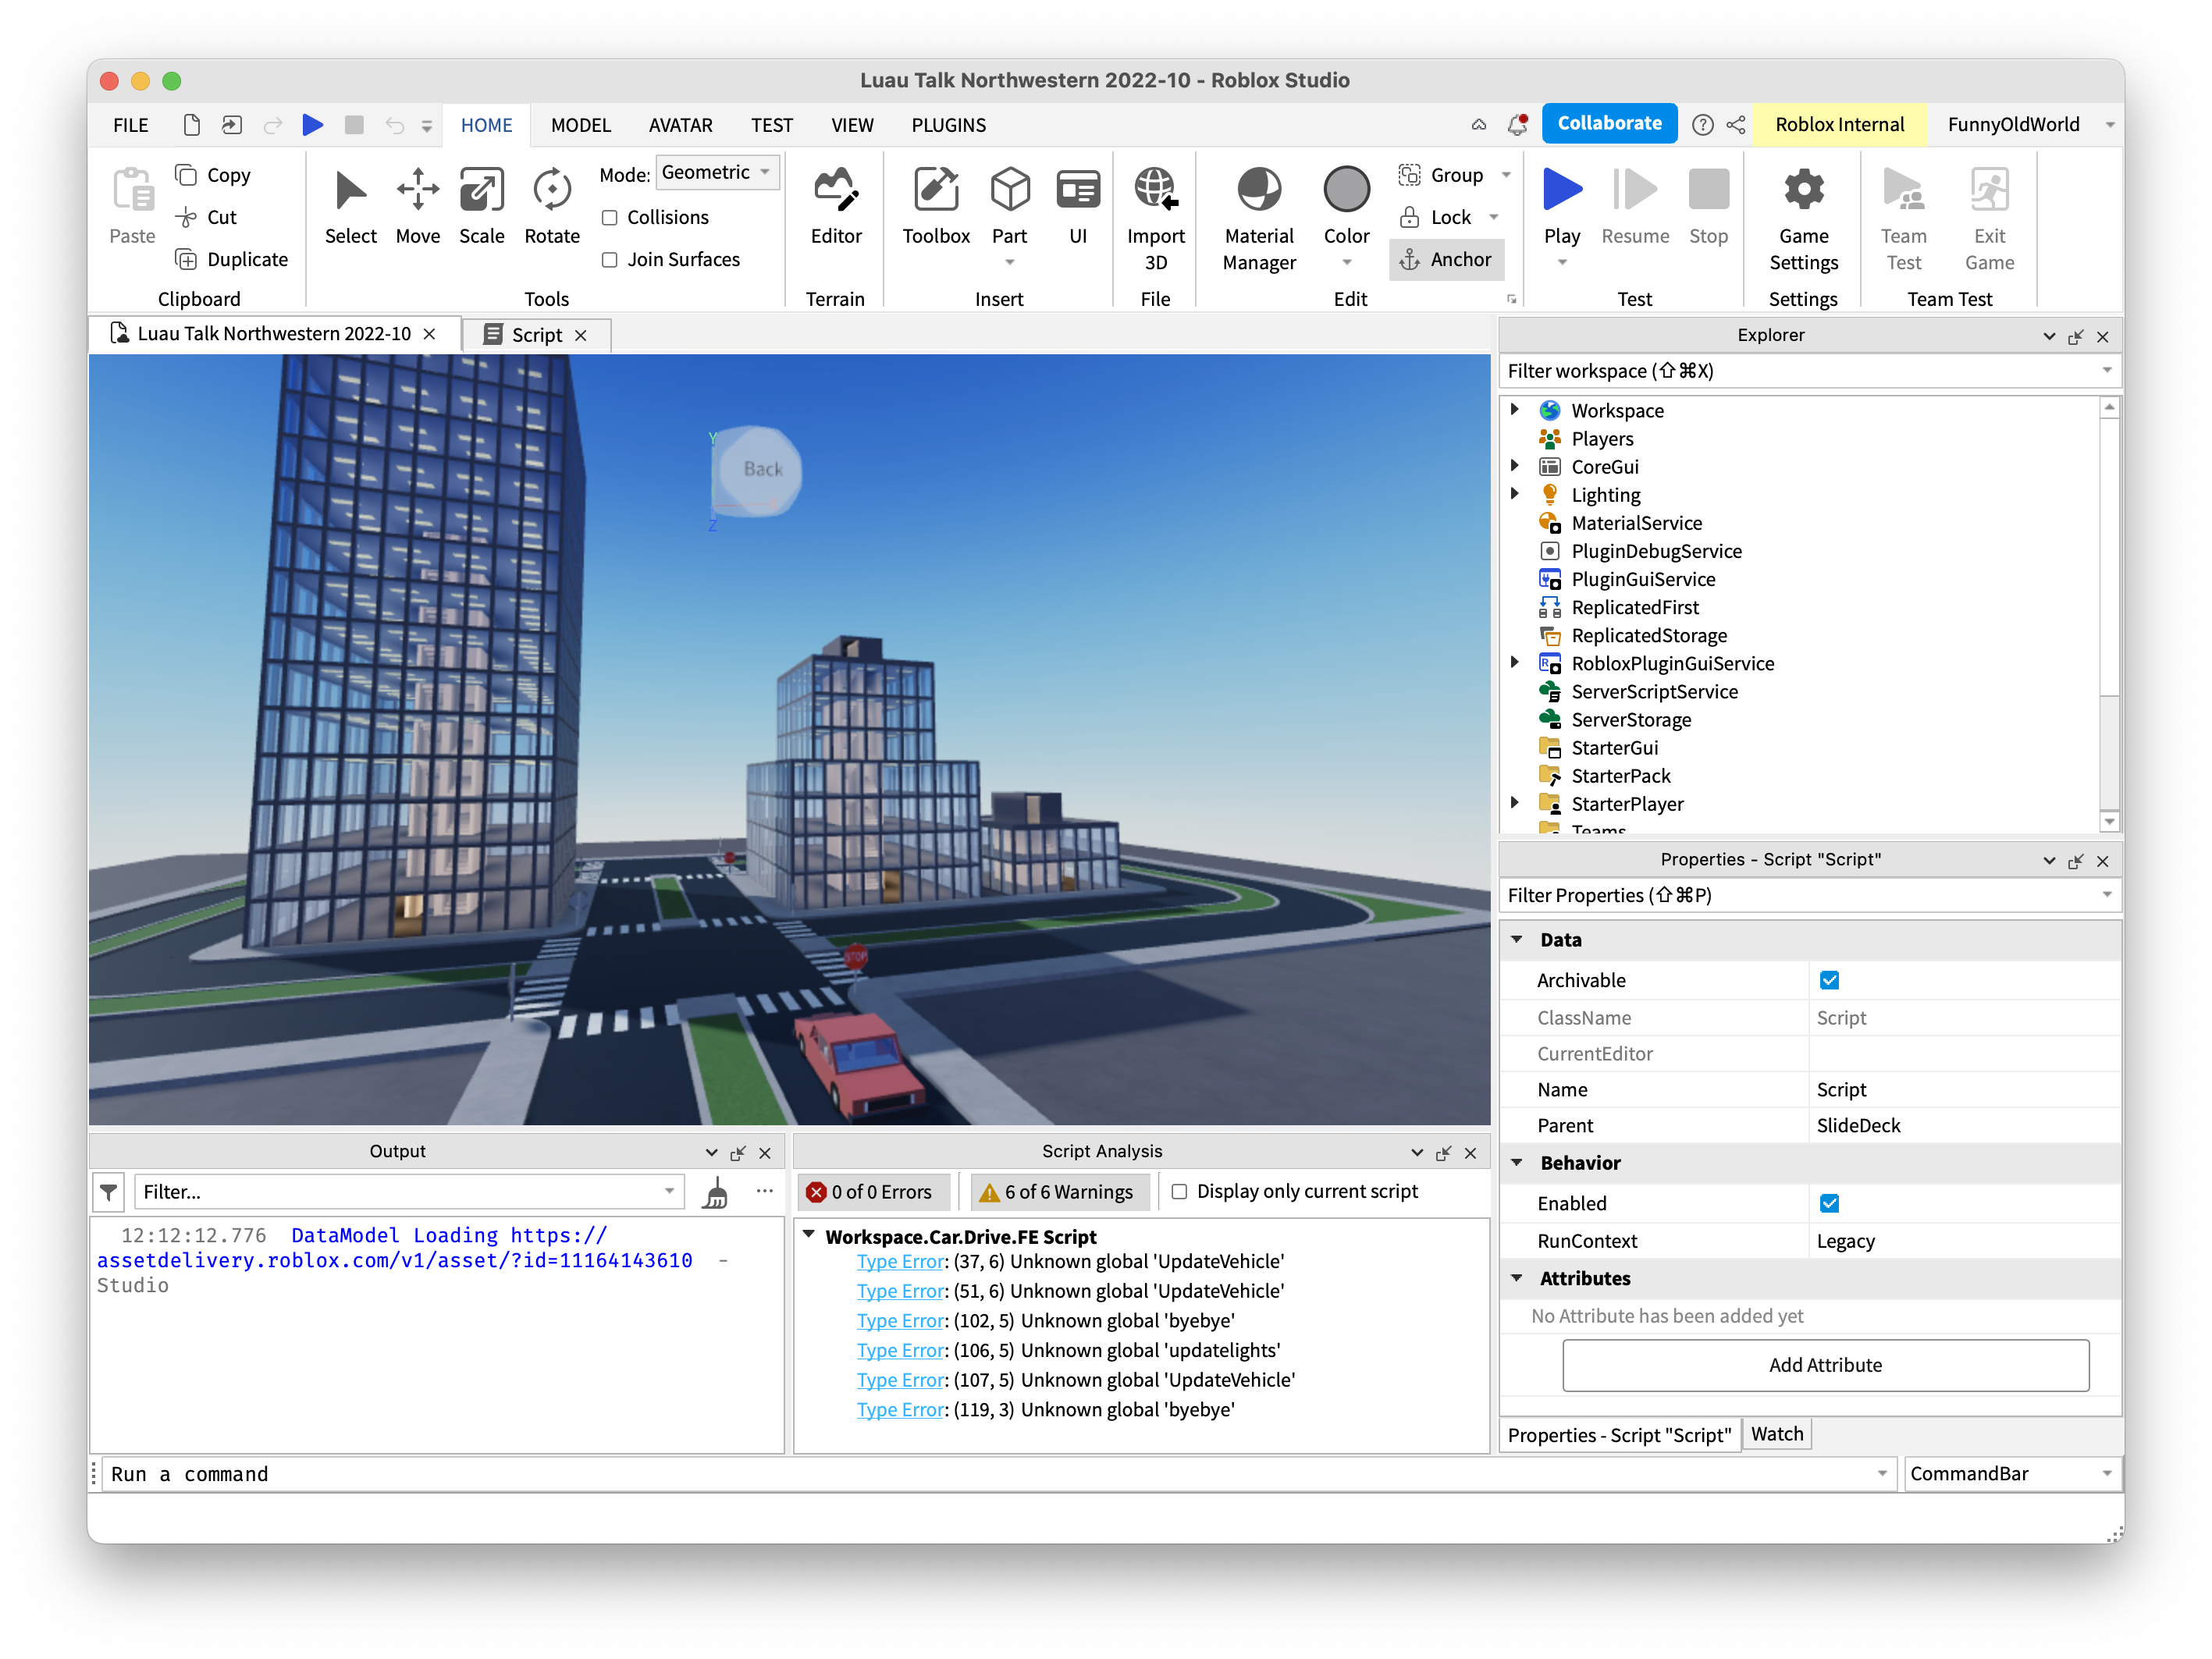
\includegraphics[width=.35\textwidth]{img/roblox-studio.png}
  \hspace{1cm}
  \includegraphics[width=.35\textwidth]{img/roblox-studio-ide.png}
  \caption{{Roblox Studio 3D creation} tools (left) and IDE (right).}
  \label{fig:roblox-studio}
\end{figure}

\Cref{t:type-error-labels} lists a few of the type errors that
script analysis can report (10 out of 35 total)
to give a sense of Luau.
A \code{SyntaxError} is the only error that can appear in
\mnocheck{} code.
Several errors in addition to \code{UnknownProperty} are about
tables, which are Luau's (and Lua's) primary data structure.
Tables support arrays, dictionaries, and objects; consequently,
tables can have methods and can usually be extended.
The error \code{TypesAreUnrelated} is a special kind of type mismatch
that arises only during cast, unification, or subtyping check.
A \code{CountMismatch} occurs when the arguments to a function
do not match the function's arity.
Similarly, an \code{IncorrectGenericParamCount} is an arity mismatch
for a generic type.
Lastly, \code{CodeTooComplex} occurs when the typechecker hits an
internal limit on problem size and \code{GenericError} is a catch-all
label for miscellaneous errors.
When Luau can provide more context regarding a generic error, it uses
a second error label called \code{ExtraInformation} to attach
a brief description.

\begin{table}
  \caption{Sample type errors.}
  % https://github.com/Roblox/luau/blob/master/Analysis/include/Luau/Error.h
  %% from type analysis, but they're not all really type errors
  \label{t:type-error-labels}

  \begin{tabular}{ll}
    Label & Interpretation \\\midrule
    \code{TypeMismatch} & Basic type error. \\
    \code{SyntaxError} & Basic parse error, e.g., \code{for if end}. \\
    \code{UnknownProperty} & Referenced an invalid field or method.  \\
    \code{OnlyTablesCanHaveMethods} & Tried to attach a method to a non-table. \\
    \code{CannotExtendTable} & Tried to extend a sealed table. \\
    \code{TypesAreUnrelated} & Failed cast, unify, or subtype. \\
    \code{CountMismatch} & Arity mismatch for a function. \\
    %% \code{CannotCallNonFunction} & Called a value that is not a function. \\
    \code{IncorrectGenericParamCount} & Arity mismatch for a generic type. \\
    \code{CodeTooComplex} & Type analysis failed, cannot understand the code. \\
    %% \code{UnificationTooComplex} & Type analysis failed, unification solver hit a limit \\
    \code{GenericError}
    & Generic label for other non-type errors, such as\\
    & \hbox{}~~looping over an unordered table.
    %% attempting to extend a type that does not describe a class
    %% attempting to iterate over a table without a clear order

  \end{tabular}
\end{table}

\paragraph{On-the-Fly Typechecking}

Scripts come in two flavors: \emph{module scripts} and \emph{non-module
scripts}.
(Though, throughout this paper we use the word ``module''
to refer to arbitrary scripts.)
Module scripts provide reusable libraries, which may be
{imported} by other scripts.
Module scripts therefore form a graph in general,
though it is an error in \mstrict{} mode to create an import cycle
and edges are removed to make the graph acyclic.
%% \QALAN{}: do all modes remove the edges?

Typechecking analyzes the entire module graph, but it also keeps track of which
modules have been edited to avoid repeating work.
Any script that the creator modifies gets marked as dirty,
and any script that is dirty or that transitively imports a dirty
module gets analyzed by the typechecker.
In the common case when typechecking is performed for autocomplete,
only the current script gets checked because it is the only dirty
script, and because nothing it requires can transitively require it, since
the module graph is acyclic.
With this strategy, the typechecker can run after every keystroke without
slowing down Roblox Studio.


\paragraph{Data Model}

The state of the world in a {Roblox} program is captured by
the \emph{data model}, which is a tree of {instances}, such as
parts, models, meshes, effects, lighting, audio assets, and physics
constraints such as forces, springs and joints.
Each asset lives in a separate file.
There may be thousands of assets.
%% The data model can be seen in the Explorer view of~\cref{fig:roblox-studio}.
%% \QALAN{} where is it? very hard to see, needs a clear label

While a program is under development, it is typical for the data
model to be edited.
% For example, instances may be added or renamed.
% --> Commented out to get a better page break.
Since the shape of the data model tree is reflected in
the type system, it is possible for these edits to introduce a mountain
of type errors across the project.


\section{Telemetry Design}

Telemetry allows an application to ``phone home'' with data
summarizing usage patterns, such performance data, crash reporting,
and feature uptake. A typical usage is in deciding whether an API can
be deprecated; without telemetry, it may be difficult to know how
popular the API is, but with telemetry it is straightforward.
Telemetry for programming languages can, however, be controversial.
See, for example, the lively discussion around telemetry in the Go
toolchain~\cite{golang-telemetry}.

Roblox Studio has a framework for reporting telemetry.
Various features in the IDE use telemetry to measure their effectiveness.
The Luau open source toolchain does \emph{not} report telemetry,
as it is designed to be used in build environments such as Continuous Integration
servers, where hermetic deterministic builds are expected.

We added a telemetry subsystem to Roblox Studio in order to study type errors
in Luau code.
This section explains the constraints our telemetry had to meet~(\cref{s:tel-limitations})
and the final design~(\cref{s:telemetry-records}).


\subsection{Limitations for Luau Telemetry}
\label{s:tel-limitations}

Telemetry in Roblox Studio faces three major constraints:
\begin{itemize}

  \item
    It \emph{must not reveal private information}.
    This can include Personally Identifying Information (PII) about creators: their identity, location, etc.
    It also includes trade secrets. Even an error message that contains the
    name of a function can reveal something the creator does not want to share.

  \item
    On the client side, telemetry computations \emph{must run quickly enough} to avoid
    slowing down the editing experience.

  \item
    Telemetry \emph{must transmit a small amount of data}---not too many records
    with not too much information inside---to avoid overloading the servers.

\end{itemize}
Cox~\cite{transparent-telemetry} discusses in detail the privacy implications
and tradeoffs in telemetry.

In addition, due to the architecture of Roblox Studio
there is some information that is not available to the
typechecker:
\begin{itemize}
  \item
    Lifecycle events including as save, run, quit, and publish.\footnote{Publish events
    cannot be reported at any rate because they are public, and could be used
    to match a telemetry session to a creator.}
  \item
    GUI state, in particular, whether the Script Analysis widget is visible.
\end{itemize}
Our type error telemetry has to meet all of the above constraints.


\subsection{Telemetry Records}
\label{s:telemetry-records}

\begin{figure}[t]\centering
  \begin{tabular}{|l|l|l|l|l|l|l|}\hline
    ID & Time & Mode & Reason & Size Info & Overall Counts & Edit Range Counts
    \\\toprule
    \multicolumn{6}{c}{\raisebox{.5\normalbaselineskip}[0pt][0pt]{$\underbrace{\hspace{9cm}}$}} &
    \multicolumn{1}{c}{\raisebox{.5\normalbaselineskip}[0pt][0pt]{$\underbrace{\hspace{3cm}}$}} \\[-0.5ex]
    \multicolumn{6}{c}{fixed-size} & \multicolumn{1}{c}{variable-size}
  \end{tabular}
  \caption{Structure of a telemetry record. There are 13 overall counts and up to 70 edit range counts in each record.}
  \label{f:tdata}
\end{figure}

The type error telemetry for a Roblox Studio session is gathered as a series of
records, all with the same \panon{} session identifier.
This allows us to correlate telemetry across a single
session, but not between sessions.
In order to avoid swamping the telemetry servers, the client reports on a subset
of telemetry events via two levels of uniform random sampling:
\begin{itemize}
  \item
    1\% of Roblox Studio sessions generate \emph{any} type error telemetry, and
  \item
    0.5\% of all type analyses (approximately 1 in 200 keystrokes)
    in an enrolled session generate a telemetry record.
\end{itemize}
In addition to sending telemetry for randomly-selected keystrokes,
our system sends a telemetry record every time the session changes
focus from one module to another.
These records provide important context for mode switches:
if one record uses \mstrict{} mode but the next uses \mnocheck{},
then it is critical to know whether the creator downgraded modes
or simply switched to another module.

\Cref{f:tdata} shows the structure of our telemetry records:
\begin{enumerate}
  \item
    ID: a \panon{} identifier for the current session.
  \item
    Time: one timestamp from the client and one from the server.
    %% timestamp explanation \cref{s:data-cleaning}
  \item
    Mode: type analysis mode of the current file: \mnocheck{},
    \mnonstrict{}, or \mstrict{}.
  \item
    Reason: a flag that explains whether this record was sent due to a
    randomly-selected keystroke or a module switch.
  \item
    Size Info: number of lines in the codebase and number of lines in the edit range.
  \item
    Overall Counts: summarizes type errors and \FS{} errors during the
    last two invocations of type analysis, and additionally reports the number
    of times type analysis hit an internal limit on problem
    size~(see~\cref{s:code-too-complex} for details).
    For each invocation and each kind of
    analysis error, there are three summary counts:
    %% grand total = 12
    \begin{itemize}
      \item total number of errors,
      \item errors in the current module, and
      \item errors in the current edit range.
    \end{itemize}
  \item
    Edit Range Counts: these list specific errors that arose in the last two
    type analyses and overlap with the current edit range.
    Since there are 35 possible errors~(\cref{s:context}), there can be up to 70 counts
    in a telemetry record.
    Exactly how to interpret this data depends on which analysis it came from:
    \begin{itemize}
      \item
        Errors in the latest type analysis are currently visible to the
        creator.
        These may have been introduced by the changes in the edit range.
      \item
        Errors from the previous type analysis were visible before the creator
        made the latest edits.
        These may have motivated some of the changes in the edit range.
    \end{itemize}
\end{enumerate}

To track the edit range, we record a start and end position, which we
update appropriately on every edit. This can result in very large and
imprecise edit ranges, for example, if the user edits at the beginning and end
of the file.
The upshot of this strategy is that it reduces the size and complexity of
telemetry records because there is only one inerval for errors to overlap with.

This telemetry design is admittedly coarse-grained.
For instance, it does not distinguish between edits that ignore a type
error from edits that remove one error while introducing another.
We acknowledge this and other threats in~\cref{s:threats}.\todo{Do we?
Double check.}
The main advantages of this telemetry are the small size of each record
and complete the lack of private information.
Furthermore, despite the limitations, this telemetry supports a variety of
interesting conclusions that we showcase in the next section.


\section{The Data}
\label{s:data}

We collected type error telemetry in Roblox Studio between February
and April 2023.
Every Studio session had a small random chance of generating
telemetry~(\cref{s:telemetry-records}).
The chosen sessions generated a record whenever the user switched modules and
randomly on each keystroke.
In total, we collected over 1.5 million telemetry records.
Roughly two thirds are due to keystrokes.

\Cref{f:records-per-hour} provides a time-ordered distribution of the data.
Each vertical bar counts the number of records generated per hour according to
a client-side timestamp.\todo{Not just per day?!?}
The bars are labeled with a California time zone.
Buckets\todo{What is a BUCKET as opposed to a BAR?}
contain a few dozen to over 3,000 records, typically about 1,000.
%% \FILL{} investigate one tower, what's happening?? all one session?
Telemetry ended in early April; the long tail is due to developers
updating Roblox Studio later.
% BEN: I see no basis for this; nor is this at all interesting.
% We do not know which timezone the records originated in, but since the counts
% tend to peak midday California time it seems that the majority
% of Roblox developers are following a Western Hemisphere schedule.
The regular pattern of the peaks suggests that many creators
follow a regular schedule; these may be
professional developers.
The tall weekend (shaded) regions could be because
Roblox has a significant school-aged creator community.

\begin{figure}[t]\centering
  %% TODO bigger text
  %% TODO weird artifact (|) in x-min label
  %% code/row-distribution.rkt
  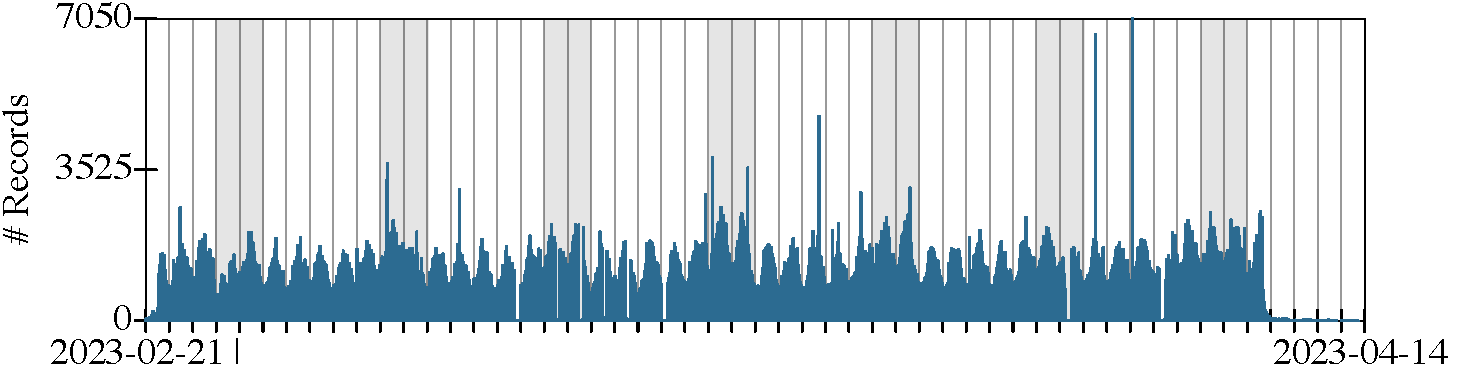
\includegraphics[width=\columnwidth]{img/row-distribution.pdf}
  \begin{tabular}{ll}
    Reason for sending:
    &
    \begin{tabular}[t]{r@{~~}l@{~~}r}
      996,164 & due to keystrokes  & [\pct{66.20}] \\
      508,572 & due to module switch & [\pct{33.80}]
    \end{tabular}
  \end{tabular}
  \caption{Telemetry records per hour. Each tick on the $x$-axis marks the start of a new day in California. Shaded ranges correspond to weekends.}
  \label{f:records-per-hour}
\end{figure}


\subsection{Data Cleaning}
\label{s:data-cleaning}

A close inspection of the data revealed two anomalies:
\begin{enumerate}
  \item
    Some records have identical timestamps and session IDs.
    We keep the first such record and discard the rest.
    (A human would have to switch modules twice or enter several keystrokes
     within 1ms to generate two such records legitimately.)

   \item
     A few hundred records~(1,533) have negative edit ranges.
     These are likely due to large deletions.
     Since the issue affects so few records, we simply ignore
     their edit ranges. We do, however, use their overall error counts and other uncorrupted fields.

\end{enumerate}

%% not important for submission
% One related observation, for which \emph{do not} sanitize the data, is
% that some records have odd timestamps according to the server's records.
% Every telemetry record comes with two timestamps: a client-side timestamp
% from when Roblox Studio created it and a server-side timestamp from when
% the server posted it to its database.
% The server timestamps are little use for our analysis because they bunch
% together; it is common for several records to have identical server
% timestamps.
% However, server timestamps are useful for auditing because they should
% be relatively close in value to the client timestamps.
% For a small number of records (<100? \FILL{}), though, the client is off by a large
% margin: up to one week behind and up to one day ahead of the server.
% We attribute the large delays to issues when sending telemetry (lost internet
% connection, etc.) and smaller offsets to incorrect time settings on the client
% machine.


\subsection{Overall Size and Shape}

Three important characteristics of the recorded data are the size of the codebases,
the length of the sessions, and the number of type
errors.
We discuss these in turn.
% Commenting these out because that's literally the rest of the
% subsection. Say anything you want from here over there!
% Codebase size and session length have long-tailed
% distributions\todo{DID YOU DO A STATISTICAL TEST.}
% with many small items and few very large ones.
% %% TODO check %% follow power-law distributions~\cite{csn-siamr-2009} 
% %% https://aaronclauset.github.io/powerlaws/
% %% bin version, is this relevant? sounds like no from abtract https://arxiv.org/pdf/1208.3524.pdf
% The number of type analysis errors is somewhat low~(explained in the next
% section), but sufficient to proceed with futher analysis.


\paragraph{Codebase Size}
%\label{s:codebase-size}

\begin{table}[t]\centering
  \caption{Size of analyzed code: number of files, number of lines, and lines in edit range}
  \label{t:codebase-size}
  % ;; (list* (max* vv) (median < vv) mm (stddev/mean mm vv) (percentile* vv)))
  % ;; percentile* = 0.95 -- 0.99
  % #hash((editrange . (1156036 926 3007043/817 30975.40553032358 (0.95 8220) (0.96 9858) (0.97 13656) (0.98 18956) (0.99 34725)))
  %       (event-count . (6079 138 38689/135 582.5752201972966 (0.95 960) (0.96 1174) (0.97 1304) (0.98 1836) (0.99 3302)))
  %       (files . (54884 7678 55257996/4639 11853.650098459446 (0.95 40029) (0.96 42771) (0.97 45417) (0.98 48688) (0.99 51761)))
  %       (lines . (1089963 3115 38928947/5992 22364.75846303099 (0.95 18561) (0.96 25892) (0.97 27014) (0.98 29725) (0.99 50547)))
  %       (timespan . (1387897376 845648 591343604248/185705 15724745.722577972 (0.95 10696064) (0.96 12715468) (0.97 15596940) (0.98 21153924) (0.99 35450460))))
  %% NOTE: 3 records have +1M lines, all from one nocheck session, all with 3 files
  %% - session "30,762,216,447,324"
  %% NOTE: 133 records have +52K files, all from one nocheck session
  %% - session "330,172,870,224,081" 
  %% (2nd biggest has 41K files "31,650,473,913,529")
%% Files has HUGE numbers thanks to data assets. Forget it.
% Files  &              &
% 11,911 & \stddev{12}  &
%  7,678 &              &
% 51,761 &              &
  \begin{tabular}[t]{lrrrrl}
    ~          & Mean  & Stddev & Median & \ptile{99} & Distribution \\
    Lines      & 6,497 & \stddev{22} & 3,115 & 50,547 & 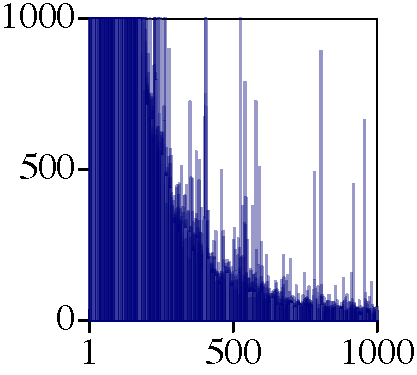
\includegraphics[width=0.14\columnwidth,valign=M]{img/lines-distribution.pdf} \\
    Edit Range & 3,680 & \stddev{31} & 926   & 34,725 & 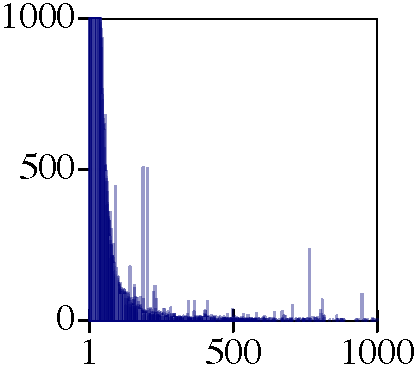
\includegraphics[width=0.14\columnwidth,valign=M]{img/editrange-distribution.pdf}
    %% TODO x-axis starts at 1, not zero
    %% TODO much bigger font or much smaller plot!!!
  \end{tabular}
\end{table}

\Cref{t:codebase-size} summarizes the size of projects in the dataset.
The four numeric columns report the mean, standard deviation, median,
and \percentile{99} for the number of lines
and lines in edit range.\footnote{The data also contains the number of files in
each project, but these numbers are difficult to relate to typechecking because
projects may contain hundreds of files that define data assets.  For the
record, the median file count is 7,678 and the \percentile{99} is 51,761 files.
}
The plots on the right show zoomed-in distributions of the line and edit range
sizes.
For example, the x-axis of the first plot counts up to 1,000 lines (not showing
a long tail to the right) and the y-axis counts up to 1,000 telemetry records
(not showing a tall spike on the left).

There is a huge amount of variation across projects.
The largest ones have over 50,000 lines of code
while the smallest have merely 1 line of code.
Unsurprisingly, these wide-ranging numbers come with large standard
deviations.
The median values are more reasonable, with roughly 3,000 lines of code
and 1,000 lines in edit ranges.


\paragraph{Session Size}
%\label{s:session-size}

\begin{table}[t]\centering
  \caption{Session size in seconds and in number of records.}
  \label{t:session-size}
  %% NOTE max time = 1 million seconds = 15 days ...  +100 are over 2 days
  \begin{tabular}{lrrrrl}
    ~               & Mean & Stddev & Median & \ptile{99} & Distribution \\
    Time Span (sec) & 3,184 & \stddev{16} & 845 & 35,450 & 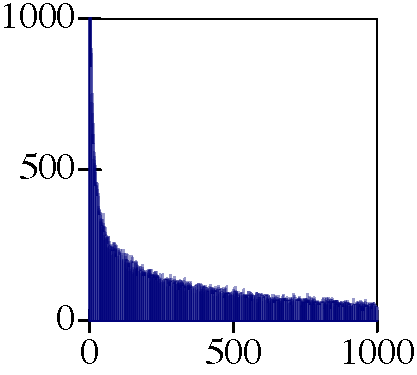
\includegraphics[width=0.14\columnwidth,valign=M]{img/timespan-distribution.pdf} \\
    Record Count    & 286 & 583         & 138 & 3,302  & 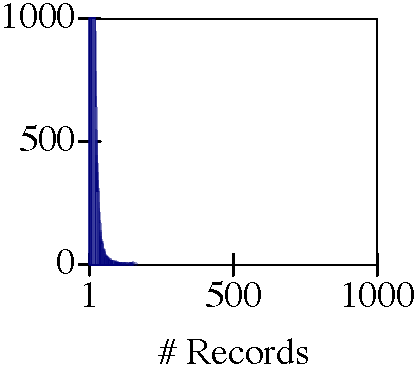
\includegraphics[width=0.14\columnwidth,valign=M]{img/event-count-distribution.pdf}
    %% TODO x-axis starts at 1
    %% TODO huge font, or smaller plot
  \end{tabular}
\end{table}

\Cref{t:session-size} similarly outlines the size of sessions using two metrics:
real time in seconds between the first and last record, and the total number of
records.
The plots focus
on the lower-left fragment of the data, which again has a very long tail.
%% comment on long-tail record counts?
The longest sessions last several days and/or contain thousands of records,
while the shortest last a few milliseconds or include just one record.
% Likewise, both plots in the figure follow a power-law distribution
% (especially for record count).
A median session runs on the order of minutes and consists of a few dozen events.
%% The median time is 14 minutes and the median 
%% The median number of records is 138.
% These numbers are reasonable.


\paragraph{Number of Type Analysis Errors}
\label{s:count-analysis-errors}

\begin{table}[t]\centering
  \caption{Current type errors and \FS{} errors across all telemetry records.}
  \label{t:count-analysis-errors}
  \begin{tabular}[t]{ll}
    \begin{tabular}[t]{r@{~~}r@{~}r}
      595,137 & type errors \\
      289,698 & \hbox{}~in module & [\pct{48.68}] \\
       30,924 & \hbox{}~in edit range & [\pct{5.20}]
    \end{tabular}
    \begin{tabular}[t]{r@{~}r@{~}r}
      72,235,735 & {\FS{} errors} \\
      37,027,281 & \hbox{}~in module & [\pct{51.26}] \\
       1,111,178 & \hbox{}~in edit range & [\pct{1.54}]
    \end{tabular}
  \end{tabular}
\end{table}

\Cref{t:count-analysis-errors} lists the number of type analysis errors
and breaks them down by location in the codebase.
In total, there are over 590,000 type errors.
The number of \FS{} errors is much larger, at 72 million, because this analysis
uses rigorous checks and runs on every module no matter what type analysis
mode the module declares.
(Furthermore, \FS{} checks run silently, so creators have no
awareness of or incentive to fix these errors.)
Approximately half the analysis errors occurred in the current module,
and a small fraction overlapped with the current edit range~(\pct{5} for
type errors, \pct{1} for \FS{}).

The large fraction of errors in the current module is encouraging
for two reasons.
First, it suggests that errors appear locally, as the result of edits to nearby
code, rather than as the result of edits to code that lives in another
module.
Second, it suggests that creators typically fix errors before switching
to another module.

The low fraction of errors in the edit range sends a mixed message:
\begin{itemize}
  \item
    On one hand, it suggests that edits successfully remove errors.
    This is true, however, only for type errors and not for \FS{} errors.
    There are 11,479 more type errors from the previous analysis
    that overlap with the current edit range~(\pct{27} difference),
    but 172,678 fewer previous \FS{} errors~(\pct{15} difference).
    Since creators can see the type errors but not the \FS{}
    errors before making edits, we conclude that the visibility
    makes a difference.
    \Cref{s:type-error-survival} explores edits and type errors in more detail.

  \item
    On the other hand, the low overlap between errors (whether current or previous)
    and edits says that edits rarely target highlighted code.
    There are several possible explanations:
    analysis might report several errors and the edits only target one or two of them;
    creators might ignore errors entirely and edit other code; or
    creators might choose to edit a non-highlighted location to fix an error.
    While non-privacy-protecting analysis have answered such
    questions~\cite{mfk-sigcse-2011}, our data cannot narrow down the answer.

\end{itemize}


\subsection{Type Analysis Modes}
\label{s:type-analysis-modes}

\begin{figure}[t]\centering
  \begin{subfigure}[b]{0.48\columnwidth}
      \begin{tabular}[t]{r@{~~}l@{~}r}
         1,341,348 & \mnocheck{}          & [\pct{89.14}] \\
           156,883 & \mnonstrict{}        & [\pct{10.43}] \\
             6,505 & \mstrict{}           & [\pct{ 0.43}]
      \end{tabular}
    \caption{Analysis modes in 1,504,736 records.}
    \label{f:total-records}
  \end{subfigure}
  \begin{subfigure}[b]{0.48\columnwidth}
      \begin{tabular}[t]{r@{~~}r@{~}r}
        313,509 & \mnocheck{}   & [\pct{90.19}] \\
         32,902 & \mnonstrict{} & [\pct{ 9.47}] \\
            545 & \mstrict{}    & [\pct{ 0.16}] \\
            642 & mixed-mode    & [\pct{ 0.18}]
      \end{tabular}
    \caption{Analysis mode(s) in 347,598 sessions.}
    \label{f:total-sessions}
  \end{subfigure}

  {Among the mixed-mode sessions:
        176 contain a mode upgrade,
        233 contain a mode downgrade, and
        512 contain modules with different modes.}

  \caption{Overview of type analysis modes.}
  \label{f:dataset-overview}
\end{figure}

Creators have three analysis modes to choose from
and can switch between modes at any time.
\Cref{f:dataset-overview} shows, however, that
usage is extremely skewed toward the default \mnocheck{} mode.
Nearly \pct{90} of all records use \mnocheck{}, while \pct{10} use
\mnonstrict{} and only a tiny fraction~(\pct{0.4}) use \mstrict{} mode.
Grouping these records into sessions shows that
\pct{90} of all sessions use \mnocheck{} exclusively,
\pct{9} use \mnonstrict{} exclusively,
and \pct{0.2} use \mstrict{} exclusively.

These adoption numbers indicate that as long as type checking is opt-in, most
creators stay opted out.
In the future, Luau plans to make \mnonstrict{} the default mode.
It will be interesting to revisit mode usage at that point.

%% mostly pure, rare mixes
Most sessions (\pct{99.82}) stick to a single analysis mode.
They never change the mode in the current module and never
switch focus to a module with a different analysis mode.
Among the other, mixed-mode sessions, most of those (\pct{80}) switch to a
module with a different mode, about half contain at least one edit that
upgrades to a more strict mode, and about half contain a downgrade to a
less-strict mode.
There are 263 total upgrades (across all sessions) and 320 total downgrades.


\paragraph{Are Upgrades Discouraging?}

%% 619 up-pairs, 583 down-pairs
%% === UP
%% min -3 max 57 median 0 mean 2.62 stddev 6.8390518952707335
%% === DOWN
%% min -48 max 30 median 0 mean -0.31 stddev 4.498748355271854

A possible explanation for the low adoption of \mnonstrict{} and
\mstrict{} mode is that upgrading to these modes leads to a large
number of type errors.
Creators might get discouraged or overwhelmed by a high error count.

The data does not support this explanation.
On average, mode-upgrades resulted in 3 additional
type errors (stddev 7, median 0).
The worst-case increase was quite high at 57 type errors, but exceptional.
In another exception, upgrading modes removed three type errors,
possibly due to other edits being rolled in with the
mode change.

In the other direction, mode downgrades have only a small negative effect on the
number of errors (mean -0.3, stddev 4, median 0, max -48).
%% curious outlier: downgrade added 30 errors!
We would see a much larger effect here if creators used downgrades
as a quick way to silence the typechecker.
But, creators evidently switch modes only when the code is already
in a well-typed state.


%% \paragraph{Module Switches vs Errors}
%% FILL need \%s out of all module switches.
%% count-modswitch in downgrade-count.rkt
%% How many module switches exit a module with errors?
%% > OLD DATA
%% > \mnocheck{} 24, \mnonstrict{} 9, \mstrict{} 3.
%% > Rare?
%% > More common for forcedstrict:
%% >  \mnocheck{} 190, \mnonstrict{} 16, \mstrict{} 2.
%% >
%% > How many module switches go to a module with errors?
%% > \mnocheck{} 70, nonstrict 9, strict 4
%% > For FS: \mnocheck{} 400, \mnonstrict{} 39, \mstrict{} 6.


\subsection{Errors by Mode}

\begin{figure}[t]\centering

  %%%% from nsa aggregate-tefs
  %% strict
  %%  te total 22771
  %%  mean 6.9 std 26.24592591869705 med 1 max 385
  %% 
  %%  fs total 114259
  %%  mean 34.9 std 155.41955823164017 med 1 max 4789
  %% 
  %% nonstrict
  %%  te total 362964
  %%  mean 2.3 std 66.44456626891912 med 0 max 13511
  %% 
  %%  fs total 7546175
  %%  mean 48.6 std 270.60578740369266 med 3 max 16712
  %%
  %% nocheck
  %%  te total 176309
  %%  mean 0.13 std 1.9040337635815197 med 0 max 289
  %% 
  %%  fs total 63784284
  %%  mean 47.7 std 885.8225471699477 med 1 max 251131

  \newcommand{\labelbars}[1]{\begin{tabular}[t]{l@{}l} \raisebox{2ex}{\begin{tabular}[t]{r}\mnocheck{}\\\mnonstrict{}\\\mstrict{}\end{tabular}} & #1 \end{tabular}}

    \begin{tabular}[t]{cc}
    %% TODO why text blurry??!
    Type errors & Background errors \\
    \labelbars{\includegraphics[width=0.20\columnwidth,valign=M]{img/error-by-mode-te.pdf}}
    & \labelbars{\includegraphics[width=0.20\columnwidth,valign=M]{img/error-by-mode-fs.pdf}}
  \end{tabular}
  \caption{Type and \FS{} errors grouped by mode.}
  \label{f:error-by-mode}
\end{figure}

Having seen the total number of errors in the dataset and the popularity of the
three analysis modes, a next question is how many errors each mode
accounts for.
There should be a few type errors in the typical \mnocheck{} record (all of
which would be syntax errors) and many more in the \mnonstrict{} and \mstrict{}
records.
For \FS{} errors, we would expect very few in \mstrict{} mode and very many in
\mnocheck{} mode.
Whereas \mnocheck{} mode performs little analysis and therefore gives fews hints
as to how to fix \FS{} errors, \mstrict{} mode checks should closely match
\FS{} checks.

\Cref{f:error-by-mode} divides errors across modes.
By the left plot, \mnonstrict{} accounts for two thirds of all type errors.
This confirms our expectation.
%% because \mnocheck{} reports only syntax errors and
%% \mstrict{} covers only a small number of telemetry records.
The right plot, by contrast, does not support our hypothesis that \mnocheck{}
records have more \FS{} errors than the other modes.
Though \mnocheck{} does have the most \FS{} errors, its \emph{proportion} matches
the proportion of \mnocheck{} records in the
dataset~(\cref{f:total-records})---if every record had exactly one \FS{} error,
the plot would be the same.

Digging further into \FS{} errors, the median number of such errors by mode is
1 in \mnocheck{}, 3 in \mnonstrict{}, and 1 in \mstrict{}.
Records in \mnocheck{} mode evidently do not have significantly more \FS{}
errors.
Furthermore, type analysis does not seem to reduce \FS{}
errors.\todo{Isn't this a bit surprising?}


\subsection{Type Errors vs. Program Edits}
\label{s:type-error-survival}

\begin{table}[t]
  \caption{Number of telemetry records that increase (\addsym{}), preserve
  (\keepsym{}), or decrease (\dropsym{}) the amount of a specific type
  error from the edit range.}
  \label{t:type-error-survival}

  \begin{tabular}{lr@{~}r@{~}rr@{~}r@{~}rr@{~}r@{~}r}
    & \zerowidth{\mnocheck{}} & & & \zerowidth{\mnonstrict{}} & & & \zerowidth{\mstrict{}} & & \\
    & \rbox{\addsym{}} & \ybox{\keepsym{}} & \gbox{\dropsym{}}
    & \rbox{\addsym{}} & \ybox{\keepsym{}} & \gbox{\dropsym{}}
    & \rbox{\addsym{}} & \ybox{\keepsym{}} & \gbox{\dropsym{}} \\\midrule
    \code{CannotCallNonFunction} & {-} & {-} & {-} & {12} & {2} & {13} & {1} & {-} & {1} \\
    \code{CannotExtendTable} & {-} & {-} & {-} & {6} & {8} & {1} & {-} & {-} & {1} \\
    \code{CannotInferBinaryOperation} & {-} & {-} & {-} & {-} & {1} & {-} & {5} & {6} & {6} \\
    \code{CountMismatch} & {-} & {-} & {-} & {184} & {42} & {157} & {9} & {2} & {9} \\
    \code{DuplicateTypeDefinition} & {-} & {-} & {-} & {1} & {-} & {-} & {-} & {-} & {-} \\
    \code{ExtraInformation} & {-} & {-} & {-} & {46} & {6} & {33} & {1} & {-} & {1} \\
    \code{FunctionDoesNotTakeSelf} & {-} & {-} & {-} & {3} & {4} & {1} & {-} & {-} & {-} \\
    \code{FunctionExitsWithoutReturning} & {-} & {-} & {-} & {6} & {1} & {5} & {7} & {3} & {5} \\
    \code{GenericError} & {-} & {-} & {-} & {177} & {47} & {149} & {5} & {-} & {8} \\
    \code{IllegalRequire} & {-} & {-} & {-} & {7} & {1} & {11} & {-} & {-} & {-} \\
    \code{IncorrectGenericParameterCount} & {-} & {-} & {-} & {-} & {-} & {-} & {1} & {-} & {1} \\
    \code{MissingProperties} & {-} & {-} & {-} & {8} & {3} & {6} & {5} & {3} & {3} \\
    \code{ModuleHasCyclicDependency} & {-} & {-} & {-} & {9} & {5} & {8} & {-} & {-} & {-} \\
    \code{NotATable} & {-} & {-} & {-} & {4} & {1} & {5} & {2} & {-} & {1} \\
    \code{OccursCheckFailed} & {-} & {-} & {-} & {-} & {-} & {-} & {-} & {-} & {1} \\
    \code{OnlyTablesCanHaveMethods} & {-} & {-} & {-} & {-} & {-} & {2} & {-} & {-} & {-} \\
    \code{OptionalValueAccess} & {-} & {-} & {-} & {21} & {45} & {15} & {4} & {2} & {4} \\
    \code{SyntaxError} & {-} & {-} & {8290} & {-} & {-} & {1149} & {-} & {-} & {29} \\
    \code{TypeMismatch} & {-} & {-} & {-} & {103} & {51} & {80} & {13} & {6} & {18} \\
    \code{UnknownPropButFoundLikeProp} & {-} & {-} & {-} & {20} & {17} & {13} & {-} & {-} & {-} \\
    \code{UnknownProperty} & {-} & {-} & {-} & {256} & {156} & {208} & {16} & {18} & {22} \\
    \code{UnknownRequire} & {-} & {-} & {-} & {43} & {30} & {37} & {5} & {3} & {3} \\
    \code{UnknownSymbol} & {-} & {-} & {-} & {1992} & {438} & {1797} & {38} & {18} & {35} \\
  \end{tabular}

\end{table}

The main focus of our telemetry design is to learn how type errors intersect
with edit ranges.
Indeed, most of the fields in a telemetry record are dedicated to this
topic~(\cref{f:tdata}), and are directed to RQ2 on type errors
(\cref{s:introduction}).

Using the results of the previous and current type analysis from
each telemetry record,~\cref{t:type-error-survival}
categorizes errors that overlap with the edit range.
The three events of interest are: when edits introduce a type
error, when edits preserve a type error, and when edits remove a
type error.
Hence, the table has three columns for each analysis mode.
In the \mnonstrict{} columns, for example, seventeen records
introduce (\addsym{}) at least one \code{CannotCallNonFunction} error.
Four records keep the number for that error at the same, nonzero level,
and twenty reduce the number of \code{CannotCallNonFunction} errors.

% BEN: double-check, I think this says all you were trying to say.
% "typically" because we COULD have gotten lucky.
The counts are imprecise because of telemetry granularity.
If a creator removes one error but then
immediately introduces another on a different line, this typically manifests as
a \keepsym{} rather than one \addsym{} and one \dropsym{}.

This table is based on the 996,164 records generated from keystroke events.
It ignores records based on module switches because those do not have
meaningful edit ranges.
One implication of the randomized strategy is that we may not notice
when a creator fixes an error; the fix must be selected by the
telemetry system.
%% \QALAN{}: what does an edit range mean for a module-switch record?
%%  there are 2 modules involved but only one range!


\paragraph{Observations}

\begin{itemize}
  \item
    The numbers in the table are low overall.
    For instance, the highest \mstrict{} count is 38
    records out of the 6,505 total~(\cref{f:dataset-overview}).
    \Cref{s:count-analysis-errors} discussions the implications
    of this low overlap rate for future work.

  \item
    \code{SyntaxError} and the related \code{UnknownSymbol} and
    \code{UnknownProperty} are most popular.
    If the edit range errors are indicative of type errors at large,
    then most errors in the data are likely due to typos.
    These errors also survive (\keepsym{}) the most often.

    Our telemetry strategy likely inflates
    the number of typos because it cannot determine when a creator is
    mid-edit.
    For example, a creator who writes a method call
    \code{bucket.countFish()} letter-by-letter will generate an
    \code{UnknownSymbol} error for \code{buck} and
    \code{UnknownProperty} for \code{bucket.c}, which may end up sampled.
    \Cref{s:conclusion} suggests ways
    to avoid this in the future.

  \item
    After the syntax errors, \code{CountMismatch}, \code{TypeMismatch}, and
    \code{GenericError} are the next most common \mnonstrict{} and \mstrict{}
    errors.
    A \code{CountMismatch} sends the wrong number of arguments to a function.
    It may simply be a common error, but it may also be a
    telemetry artifact.
    The high incidence of \code{TypeMismatch} and \code{GenericError} calls for
    further study in future work to determine precisely which error arose.
    (Some of the \code{GenericError}s come with context strings in the form of
    \code{ExtraInformation} errors, but telemetry does not report these strings.)
    %% GenericError = only a few things: extend non-class, iterate non-table, ...?

  \item
    \code{OptionalValueAccess} frequently persists through edits (\keepsym{}).
    Creators may be ignoring this error because they can deduce that the
    optional value will be present at runtime.

  \item
    %% Drop >= Add >= Rem ~= 18
    %% other nonzero      ~= 21 triples
    Ideally, the highest number in each column group should
    be decreases (\dropsym{}).
    A decrease should happen when the creator sees an error and
    fixes it.
    However, decreases are highest in only 18 of the 39 nonzero groups.

%%  \item
%%    \FILL{} \mnonstrict{} should have no false positives,
%%    \mstrict{} doesn't care.
%%    Why so many keeps in NS??!

%%  \item
%%    A few errors are more common in \mstrict{} than \mnonstrict{}:
%%    \code{CannotInferBinaryOperation},
%%    \code{FunctionExitsWithoutReturn},
%%    \code{IncorrectGenericParamCount}.
%%    \FILL{} so what.

%%   \item
%%     (NOTE may want to save relative popularity for next section.)
%%     Some errors occur more often in \mnonstrict{} than \mstrict{}:
%%     \code{CannotCallNonFunction},
%%     \code{CannotExtendTable},
%%     \code{GenericExtraInformation},
%%     \code{FunctionDoesNotTakeSelf},
%%     \code{IllegalRequire},
%%     \code{ModuleHasCyclicDependency},
%%     \code{OptionalValueAccess},
%%     \code{UnknownPropButGotLikeProp}.
%%     \QALAN{} are any of these surprising, or expected from the bigger number of
%%     \mnonstrict{} records?

\end{itemize}



\subsection{Type Error Popularity}
\label{s:type-error-count}

\begin{table}[t]\centering
  %% NOTE: popularity looks similar when [over all records] vs. [restricted to module switch records]
  \caption{Type error popularity for \mnonstrict{} and \mstrict{} modes.}
  %% {(all of the type errors in \mnocheck{} mode are \code{SyntaxError}s).}
  \label{t:type-error-count}
  \begin{tabular}{ll}
    \mnonstrict{} & \mstrict{} \\
    \begin{tabular}[t]{l@{~}r}
      \code{UnknownSymbol} & \pct{62.13} \\
      \code{SyntaxError} & \pct{15.42} \\
      \code{UnknownProperty} & \pct{8.28} \\
      \code{UnknownRequire} & \pct{3.13} \\
      \code{TypeMismatch} & \pct{2.44} \\
      \code{CountMismatch} & \pct{2.26} \\
      \code{OptionalValueAccess} & \pct{2.07} \\
      \code{GenericError} & \pct{2.06} \\
      \code{UnknownPropButGotLikeProp} & \pct{0.44} \\
      \code{CannotExtendTable} & \pct{0.42} \\
      \code{GenericExtraInformation} & \pct{0.32} \\
      \code{ModuleHasCyclicDependency} & \pct{0.23} \\
      \code{IllegalRequire} & \pct{0.20} \\
      \code{NotATable} & \pct{0.15} \\
      \code{CannotCallNonFunction} & \pct{0.15} \\
      \code{MissingProperties} & \pct{0.09} \\
      \code{FunctionExitsWithoutReturn} & \pct{0.07} \\
      \code{FunctionDoesNotTakeSelf} & \pct{0.07} \\
      \code{MissingUnionProperty} & \pct{0.02} \\
      \code{CannotInferBinaryOperation} & \pct{0.02} \\
      \code{OnlyTablesCanHaveMethods} & \pct{0.01} \\
      \code{DuplicateTypeDefinition} & {<\pct{0.01}} \\
      \code{TypesAreUnrelated} & {<\pct{0.01}} \\
    \end{tabular}
        &
    \begin{tabular}[t]{l@{~}r}
      \code{UnknownSymbol} & \pct{23.97} \\
      \code{TypeMismatch} & \pct{20.46} \\
      \code{UnknownProperty} & \pct{18.88} \\
      \code{SyntaxError} & \pct{9.31} \\
      \code{CannotInferBinaryOperation} & \pct{6.94} \\
      \code{MissingProperties} & \pct{4.04} \\
      \code{CountMismatch} & \pct{2.99} \\
      \code{OptionalValueAccess} & \pct{2.99} \\
      \code{FunctionExitsWithoutReturn} & \pct{2.99} \\
      \code{UnknownRequire} & \pct{2.37} \\
      \code{GenericError} & \pct{2.28} \\
      \code{NotATable} & \pct{1.32} \\
      \code{GenericExtraInformation} & \pct{0.35} \\
      \code{UnknownPropButGotLikeProp} & \pct{0.26} \\
      \code{IncorrectGenericParamCount} & \pct{0.18} \\
      \code{CannotCallNonFunction} & \pct{0.18} \\
      \code{IllegalRequire} & \pct{0.18} \\
      \code{ModuleHasCyclicDependency} & \pct{0.09} \\
      \code{CannotExtendTable} & \pct{0.09} \\
      \code{OccursCheckFailed} & \pct{0.09} \\
      \code{TypesAreUnrelated} & \pct{0.09} \\
    \end{tabular}
  \end{tabular}
\end{table}

%% UNUSED CODES
%% \mnonstrict{}
%%   CodeTooComplex
%%   DeprecatedApiUsed
%%   DuplicateGenericParameter
%%   DynamicPropertyLookupOnClassesUnsafe
%%   FunctionRequiresSelf
%%   IncorrectGenericParameterCount
%%   InternalError
%%   NormalizationTooComplex
%%   OccursCheckFailed
%%   SwappedGenericTypeParameter
%%   TypePackMismatch
%%   UnificationTooComplex
%% 
%% \mstrict{}
%%  CodeTooComplex
%%  DeprecatedApiUsed
%%  DuplicateGenericParameter
%%  DuplicateTypeDefinition
%%  DynamicPropertyLookupOnClassesUnsafe
%%  FunctionDoesNotTakeSelf
%%  FunctionRequiresSelf
%%  InternalError
%%  MissingUnionProperty
%%  NormalizationTooComplex
%%  OnlyTablesCanHaveMethods
%%  SwappedGenericTypeParameter
%%  TypePackMismatch
%%  UnificationTooComplex

%% both NS S
%%  CodeTooComplex
%%  DeprecatedApiUsed
%%  DuplicateGenericParameter
%%  DynamicPropertyLookupOnClassesUnsafe
%%  FunctionRequiresSelf
%%  InternalError
%%  NormalizationTooComplex
%%  OnlyTablesCanHaveMethods
%%  SwappedGenericTypeParameter
%%  TypePackMismatch
%%  UnificationTooComplex

\Cref{t:type-error-count} reports the percent of type errors that overlap with
the edit range.\todo{I DO NOT UNDERSTAND ANYTHING HERE.}
The purpose of this table is to discover all specific errors in the dataset,
thus it includes both keystroke-based and module-switch-based records---even
though edit ranges are not well-defined for the latter.

There are two subtables for \mnonstrict{} and \mstrict{} mode.
The table does not report \mnocheck{} because all its type errors are
by definition \code{SyntaxError}s.


\paragraph{Observations}

\begin{itemize}
  \item
    Syntax errors, in particular \code{UnknownSymbol}, are much more
    common in \mnonstrict{} than \mstrict{}.\todo{This is NOT a
      ``syntax'' error? It's a typo!}
    This may be because \mnonstrict{} reports fewer errors in general.

  \item
    Despite being less strict, \mnonstrict{} reported four errors that
    never appeared in the \mstrict{} records:
    \code{DuplicateTypeDefinition}, \code{OnlyTablesCanHaveMethods},
    \code{MissingUnionProperty}, and \code{FunctionDoesNotTakeSelf}.
    We attribute this to the much larger number of \mnonstrict{} records in the
    dataset.

  \item
    \code{TypeMismatch} is far more common in \mstrict{} (\pct{20.46})
    than \mnonstrict{} (\pct{2.44}) because \mstrict{} mode
    has additional type constraints.
    Several other errors have higher \mstrict{} percentages for the
    same reason, such as \code{CannotInferBinaryOperation}, and
    two errors appeared only in \mstrict{}:
    \code{OccursCheckFailed} and \code{IncorrectGenericParamCount}.

  \item
    Several Luau errors never appeared in edit ranges.
    Four of these deal with internal typechecker limits, which we discuss
    below.
    The others are for: dynamic property lookups,
    deprecated APIs, swapped generic parameters,
    functions that require a self, and type pack mismatches.
    We would not expect these to appear often.

    % \code{DynamicPropertyLookupOnClassesUnsafe},
    % \code{SwappedGenericTypeParameter},
    % \code{DeprecatedApiUsed},
    % \code{DuplicateGenericParameter},
    % \code{FunctionRequiresSelf}, and
    % \code{TypePackMismatch}.

\end{itemize}

\paragraph{Internal Limits, Code Too Complex}
\label{s:code-too-complex}
%% data = out/ctc-info.txt

To deal with pathologies such as the worst-case time for ML-style type
inference~\cite{m-popl-1990,ktu-caap-1990}, the typechecker
has internal limits that restrict the problems it will attempt to solve.
Hitting a limit triggers one of the following errors:
\code{CodeTooComplex},
\code{NormalizationTooComplex}, or
\code{UnificationTooComplex}.
These errors can appear in Script Analysis just like any other
error, but one design goal of Luau is that code rarely hits the limits.
A typical creator should never see these errors.

Fortunately, the data rarely contains too-complex errors.
None of these errors appear in edit ranges~(\cref{t:type-error-count}).
For the specific case of \code{CodeTooComplex}, our telemetry tracked project-wide
counts and found only 26 errors, which were spread across eleven
records in three sessions.
Note that all three sessions \emph{could} have been from the same codebase.
% BEN: I see no reason for this speculation. The only important thing
% is the fact that this could have been all the same codebase.
%It is entirely possible that they all came from one session that
%deliberately pushed the limits of type analysis.
%% Whatever the reason, the overall number is low enough to suggest that the
%% internal limits are not posing barriers to typechecker adoption.


\subsection{Density of Type Errors}

\begin{figure}[t]\centering
  %% FS plots look similar
  %% - much higher densities, same basic story
  %% - nocheck indeed the highest > NS > S
  %% TODO draw units, bigger font

  \mnocheck{}
  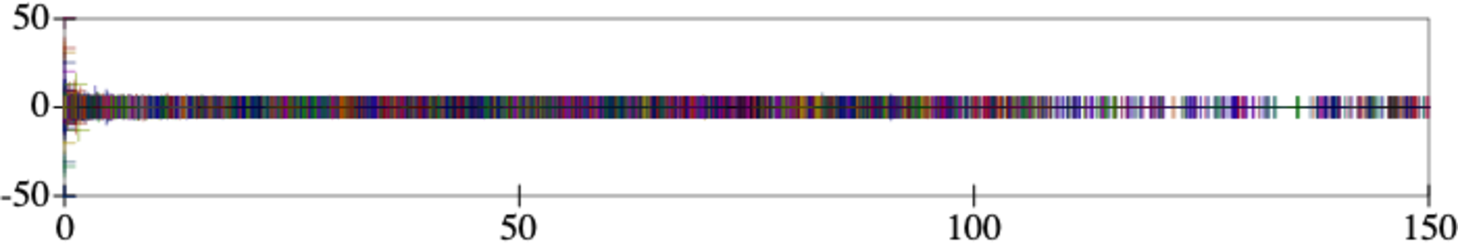
\includegraphics[width=\columnwidth]{img/error-count-nocheck-row--te-density-diff.pdf}

  \mnonstrict{}
  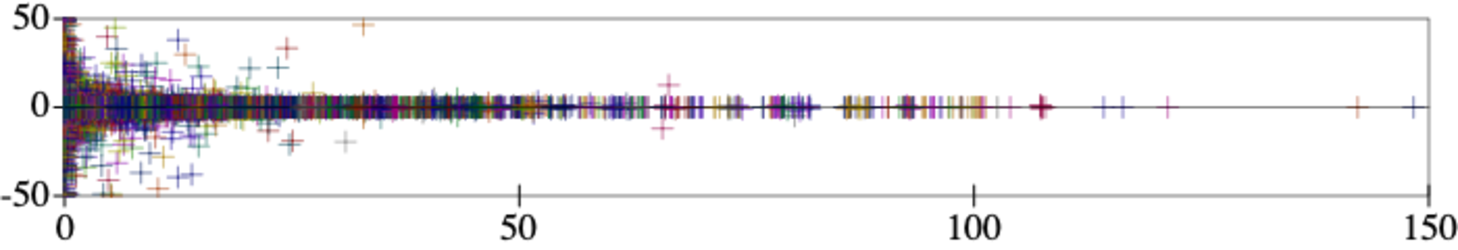
\includegraphics[width=\columnwidth]{img/error-count-nonstrict-row--te-density-diff.pdf}

  \mstrict{}
  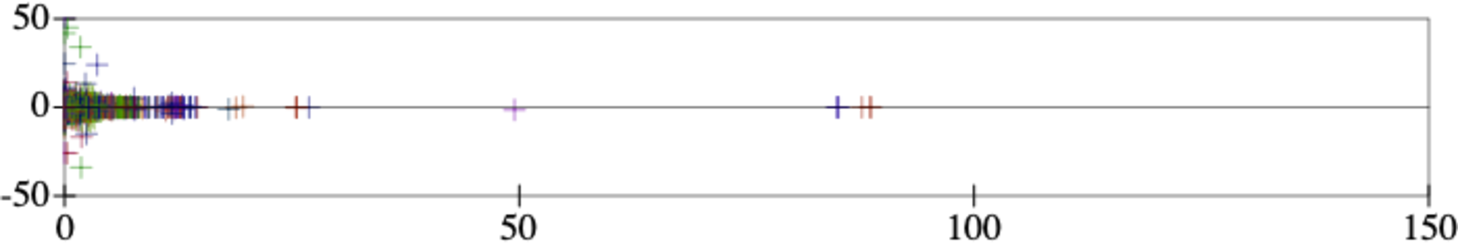
\includegraphics[width=\columnwidth]{img/error-count-strict-row--te-density-diff.pdf}
  \caption{Changes in type error density (errors / lines) over time (seconds).}
  \label{f:error-density}
\end{figure}

Since errors and edits may not overlap, either because the highlights
are misleading or because the creator ignores the errors, it is important
to see how the total errors change over time.
We measure \emph{error density} rather than error count, however,
to normalize for the wide range of codebase sizes~(\cref{t:codebase-size}).
Density is the number of type errors divided by the number of lines.

\Cref{f:error-density} plots changes to error density for every session in the dataset.
The x axis counts time in seconds from the start of the session.
Most sessions last a few dozen seconds~(\cref{t:session-size}), so the axis
ends at 150 seconds.
The y axis shows changes to errors over time; a positive number means errors
increased since the last record, and a negative number represents a decrease.
While there are a few errors that go outside the plot bounds
(max \mnocheck{}: 101, max \mnonstrict{}: 3577, max \mstrict{}: 87), we focus
on $\pm{}50$ errors because most of the mass is in that region.
The points are color-coded to give each session the same color, but this is not
very useful because there are many more sessions than colors.


\paragraph{Observations}

% Due to the relative adoption of type analysis, there is much more
% data for the weak \mnocheck{} mode than for \mnonstrict{},
% and in turn for \mnonstrict{} relative to \mstrict{}.
% Still, the plots reveal interesting points:

\begin{itemize}
  \item
    All three plots are roughly balanced,
    with equal ``mass'' above and below the x-axis.
    The next section explores this point in detail.

  \item
    After the 40-second mark, changes to type error density become much
    smaller.
    These long-running sessions are not introducing errors.
    %% TODO check #mod switch in long sessions

  \item
    \mnonstrict{} has the biggest fluctuations in errors, whereas \mstrict{}
    has the smallest.
    One explanation is that some \mnonstrict{} sessions ignore type analysis
    (in particular the one with over 3,000 errors!) whereas most \mstrict{}
    sessions pay close attention to it.

  %% \item
  %%   TODO plot FS with a much bigger range ... tells a different story about buildup?

\end{itemize}


\subsection{Do Edits Tend to Add Type Errors?}
\label{s:tefs-compass}

\begin{figure}[t]\centering
  % TODO use bars instead, percent only, don't care about counts

  % TE: nocheck & 48378 & [\pct{46.83}] & 9440 & [\pct{9.14}] & 45479 & [\pct{44.03}] \\
  % TE: nonstrict & 19491 & [\pct{39.63}] & 9567 & [\pct{19.45}] & 20121 & [\pct{40.91}] \\
  % TE: strict & 733 & [\pct{39.18}] & 368 & [\pct{19.67}] & 770 & [\pct{41.15}] \\
  %
  % TE mod: nocheck & 20085 & [\pct{49.83}] & 906 & [\pct{2.25}] & 19317 & [\pct{47.92}] \\
  % TE mod: nonstrict & 13030 & [\pct{40.22}] & 5513 & [\pct{17.02}] & 13852 & [\pct{42.76}] \\
  % TE mod: strict & 419 & [\pct{39.31}] & 230 & [\pct{21.58}] & 417 & [\pct{39.12}] \\
  %
  % FS: nocheck & 270763 & [\pct{36.99}] & 238696 & [\pct{32.61}] & 222588 & [\pct{30.41}] \\
  % FS: nonstrict & 35330 & [\pct{37.28}] & 29483 & [\pct{31.11}] & 29955 & [\pct{31.61}] \\
  % FS: strict & 574 & [\pct{33.71}] & 561 & [\pct{32.94}] & 568 & [\pct{33.35}] \\
  %
  % FS mod: nocheck & 259865 & [\pct{39.09}] & 175643 & [\pct{26.42}] & 229271 & [\pct{34.49}] \\
  % FS mod: nonstrict & 33988 & [\pct{39.74}] & 20738 & [\pct{24.25}] & 30798 & [\pct{36.01}] \\
  % FS mod: strict & 488 & [\pct{36.53}] & 344 & [\pct{25.75}] & 504 & [\pct{37.72}] \\
  \begin{tabular}{l@{~~}lr@{}rr@{}rr@{}r}
    & & \zerowidth{\rbox{\addsym{}}} & & \zerowidth{\ybox{\keepsym{}}} & & \zerowidth{\gbox{\dropsym{}}} \\\midrule
    type      & \mnocheck{}   & 20085 & [\pct{49.83}] & 906 & [\pct{2.25}] & 19317 & [\pct{47.92}] \\
    error     & \mnonstrict{} & 13030 & [\pct{40.22}] & 5513 & [\pct{17.02}] & 13852 & [\pct{42.76}] \\
              & \mstrict{}    & 419 & [\pct{39.31}] & 230 & [\pct{21.58}] & 417 & [\pct{39.12}] \\
    \\[-2ex]
    \FS       & \mnocheck{}   & 259865 & [\pct{39.09}] & 175643 & [\pct{26.42}] & 229271 & [\pct{34.49}] \\
    error     & \mnonstrict{} & 33988 & [\pct{39.74}] & 20738 & [\pct{24.25}] & 30798 & [\pct{36.01}] \\
              & \mstrict{}    & 488 & [\pct{36.53}] & 344 & [\pct{25.75}] & 504 & [\pct{37.72}] \\
  \end{tabular}
  \caption{How often do edits increase, maintain, or decrease the number of errors?}
  \label{f:error-changes}
\end{figure}

The visual symmetry in the density plots~(\cref{f:error-density})
suggests that edits add and remove errors with rougly equal frequency,
regardless of mode.
\Cref{f:error-changes} explores this question of balance in detail.
For each of the three modes, it reports the percent of edits that increase (\addsym{}),
maintain (\keepsym{}), or decrease (\dropsym{}) the number of type
errors in the module.
It also reports counts for \FS{} checks to see whether fixing type errors fixes
\FS{} errors as well.
The ``maintain'' rows include cases where there are zero errors before and after.


\paragraph{Observations}

\begin{itemize}
  \item
    The type error increases and decreases are remarkably balanced: across all
    three modes, they are at most \pct{2} apart.
    While some of this balance is due to module-switch records
    (if the two modules have different error counts, there will be a change),
    most of the data is from keystrokes; thus, it appears that sessions tend to
    fix errors highlighted by type analysis.

  \item
    \mstrict{} mode has a higher percent of ``maintain'' (\keepsym{}) records.
    Errors may be more likely to persist in this mode.
    %% TODO check if actually zero

  \item
    In \FS{} mode, the percent of ``maintain'' records is high across
    the board and the increases and decreases are lower.
    No matter the mode, reducing type errors is not guaranteed to reduce
    \FS{} errors as well.
    This is surprising for \mstrict{} mode, and likely relates to
    the data model; see below for details.

\end{itemize}


\paragraph{Data Model Types: Strict vs. Background Analysis}

Based on the description of \FS{} analysis from~\cref{s:context},
it should raise \emph{at least as many errors} as \mstrict{} mode
because it uses \mstrict{} checks for all dependencies.
For example, if a \mstrict{} module imports from a \mnocheck{} one,
then \mstrict{} analysis does not analyze the import but
\FS{} analysis does.

In \cref{f:error-changes}, however, nearly \pct{3} of \mstrict{}-mode records
increase the number of \mstrict{} errors without increasing \FS{} errors.
Further inspection reveals that the situation is a bit worse, as
some records increase \mstrict{} errors without changing the \FS{} errors:
    \pct{22} of \mstrict{} records increase (\addsym{}) the number of type errors
    but maintain (\keepsym{}) the number of \FS{} errors.

The reason for the discrepancy is that \mstrict{} mode and \FS{} analysis
assign different types to the data model: \mstrict{} assigns a top type
and requires downcasts at use sites, whereas \FS{} analysis uses the
dynamic gradual type.
Dealing with these data model errors may be a source of frustration
for creators using \mstrict{} mode.


\section{Answers to Research Questions}
\label{s:discussion}

With the data in hand, we can answer the research questions
from~\cref{s:introduction}.
The answers confirm several aspects of Luau's design, but
at the same time offer several directions for future improvements.

Luau clearly\todo{How can we say?} has a powerful typechecker that can efficiently
analyze thousands of lines of code.
But, few sessions use type analysis directly and the data presents little
evidence that doing so would improve creators' quality of life.
We conjecture that Luau needs further tailoring to match
common idioms in Roblox scripts.
Discovering these idioms is a question for future work~(\cref{s:conclusion}).

\begin{description}
  \item[How many sessions use type analysis?]
    A mere \pct{10} of sessions (and of telemetry records overall) opt-in to
    type checking~(\cref{f:dataset-overview}).
    Most of these use \mnonstrict{} mode, and fewer than \pct{1}
    use \mstrict{} mode.

  \item[How often do projects contain modules with different analysis modes?]
    Sessions rarely combine analysis modes.
    Only 512 of \nK{340} sessions ($<\pct{0.15}$) switched to modules with different
    analysis modes.
    This number may be a significant underapproximation because we have data
    only on modules that the creator chose to open, but the widespread use
    of \mnocheck{} mode suggests that it is not off by much.

  \item[How often do sessions turn analysis off?]
    Sessions rarely disable type analysis after opting in.
    Only 233 of the \nK{340} sessions ($<\pct{0.07}$)
    switch to a weaker mode.
    One-fourth of the downgrades switch from \mstrict{}
    to \mnonstrict{}, and therefore keep some type analysis.
    The remainder switch from \mstrict{} to \mnocheck{} (\pct{50})
    or from \mnonstrict{} to \mnocheck{} (\pct{25}).
    %% FILL more insight if we match ups and downs together??

    %% upgrade
    %% 519 total sessions
    %% 176 with up
    %% 263 total up
    %% #hash((nocheck . 0) (nonstrict . 44) (strict . 132))
    %%  nocheck : 0.00\%
    %%  strict : 75.00\%
    %%  nonstrict : 25.00\%
    %%%% #hash(((strict nocheck) . 88)
    %%%%       (nonstrict . 0)
    %%%%       (strict . 0)
    %%%%       ((nonstrict nocheck) . 44)
    %%%%       (nocheck . 0)
    %%%%       ((strict nonstrict) . 44))
    %%%%  (strict nonstrict) : 25.00\%
    %%%%  nocheck : 0.00\%
    %%%%  (nonstrict nocheck) : 25.00\%
    %%%%  strict : 0.00\%
    %%%%  nonstrict : 0.00\%
    %%%%  (strict nocheck) : 50.00\%
    %%
    %% downgrade
    %% 515 total sessions
    %% 233 with down
    %% 320 total down
    %% #hash((nocheck . 0) (nonstrict . 64) (strict . 169))
    %%  nocheck : 0.00\%
    %%  strict : 72.53\%
    %%  nonstrict : 27.47\%
    %%%% #hash(((strict nocheck) . 116)
    %%%%       (nonstrict . 0)
    %%%%       (strict . 0)
    %%%%       ((nonstrict nocheck) . 64)
    %%%%       (nocheck . 0)
    %%%%       ((strict nonstrict) . 53))
    %%%%  (strict nonstrict) : 22.75\%
    %%%%  nocheck : 0.00\%
    %%%%  (nonstrict nocheck) : 27.47\%
    %%%%  strict : 0.00\%
    %%%%  nonstrict : 0.00\%
    %%%%  (strict nocheck) : 49.79\%




  \item[For modules that use type analysis (\mstrict{} and \mnonstrict{}):]\leavevmode
    \begin{description}
      \item[- Which errors arise?]
        Syntax errors are extremely common~(over \pct{50},~\cref{t:type-error-count}), 
        followed by type mismatches~(\pct{20} in \mstrict{}),
        arity errors~(\pct{2}),
        and failure to unpack on optional value~(\pct{2}).
        There are several uncommon errors, such as misusing a table operation,
        and a few that never arise: internal and too-complex errors,
        duplicating or swapping a generic parameter, use of a deprecated API,
        and unsafe dynamic property lookup on a class.

      \item[- How do sessions respond? Which errors persist through edits?]
        Sessions typically fix analysis errors.
        With few exceptions, increases and decreases in the number of errors
        balance out~(\cref{f:error-changes,t:type-error-survival,}).
        Even in \mnocheck{}, most edits that overlap with syntax errors
        remove at least one error~(\pct{67}) rather than increase or maintain
        the total.
        The errors that most often survive edits are due to
        inference at a binary operation,
        sending \code{self} to a function that does not expect it,
        and failure to unpack an optional value.
        But the first two seldom arise, and the third is something creators
        might reasonably ignore while prototyping.

%% Keep percents
%% '((CannotInferBinaryOperation "0.50")
%%   (OptionalValueAccess "0.44")
%%   (FunctionDoesNotTakeSelf "0.40")
%%   (CannotExtendTable "0.35")
%%   (UnknownPropButGotLikeProp "0.28")
%%   (UnknownProperty "0.26")
%%   (MissingProperties "0.25")
%%   (FunctionExitsWithoutReturn "0.21")
%%   (ModuleHasCyclicDependency "0.20")
%%   (UnknownRequire "0.18")
%%   (TypeMismatch "0.18")
%%   (UnknownSymbol "0.15")
%%   (NotATable "0.12")
%%   (GenericError "0.11")
%%   (CannotCallNonFunction "0.10")
%%   (CountMismatch "0.09")
%%   (GenericExtraInformation "0.07")
%%   (IllegalRequire "0.06")
%%   (SyntaxError "0.01")

    \end{description}

  \item[What impact does type analysis have on the number of \FS{} errors?]
    Opting in to type analysis has little impact on \FS{} errors.
    The percent of \FS{} errors in \mnocheck{} code matches the percent of
    sessions using \mnocheck{} mode~(\cref{f:error-by-mode}); whereas,
    if type analysis helped reduce \FS{} errors, \mnocheck{} would own a
    higher percentage of the errors.
    Furthermore, there is no apparent relation between \FS{} errors and edits,
    regardless of analysis mode~(\cref{f:error-changes}).
    A randomly-chosen edit has a 1/3 chance of increasing, decreasing, or
    maintaining the number of \FS{} errors.

\end{description}


\paragraph{Threats to Validity}
\label{s:threats}

While this study has high ecological validity due to its focus on
working creators, there are several threats to keep in mind.
Some threats stem from our method of collecting data; others
come from the limited scope of the data.

First of all, sampling is necessarily incomplete.
Though the data includes many thousands of sessions, it
may have missed a few critical sessions where a creator
adopted \mstrict{} mode, encountered \code{CodeTooComplex} errors,
and gave up.
Furthemore, our method of sampling by keystroke and by module switch
skews the data toward creators who, for whatever reason, do more
of these actions.
We have no access to other events, e.g., run locally~(\cref{s:tel-limitations});
future studies may wish to avoid this limitation by actively
recruiting subjects.

Second, the edit ranges are a coarse approximation of actual edits.
They begin at the lowest edited line of code and end at the highest
edited line, even if nothing between those lines changed.

Third, session-based data has limitations.
A creator who closes and reopens Roblox Studio every day has
a much higher chance of generating telemetry than one who
leaves Studio open all week.
We have no way to reliably check whether multiple sessions are
reporting on the same codebase.
Sessions may end abruptly, for instance because of machine reboot,
instead of ending when the creator was finished editing code.

Fourth, the total counts of type errors include a large number of syntax errors,
which have little to do with the Luau type system and are presumably easy for
creators to fix.
It would be better for the analysis to ignore these errors.
Indeed, our comparison between \FS{} errors in \mnocheck{} vs.
\mstrict{} mode~(\cref{f:error-changes}) might tell a very different story
without all the noise that syntax errors introduce.\todo{Why didn't
  YOU just filter them, then?!?}

Fifth, type analysis reports several errors at once and we have no idea which
errors, if any, creators intended to fix with their edits.
Thus, fixes may be a side effect of other plans, as seen in prior work~\cite{mfk-sigcse-2011}.
% This is the [DIFF] code from Marceau SIGCSE 2011.

% Telemetry cannot replace user studies, as there is no way to measure
% creator sentiment, but provide complementary data at scale.
% No idea about intent is a big problem, we don't know which error the creator wanted to fix.

Lastly, we have two remarks about external validity.
First, our information on type errors is limited to error names.
If another language has an error that is roughly similar to
the\todo{Huh? It's similar yet different?}
\code{CannotCallNonFunction} error but with slightly different
semantics, then the relative frequency of that error could be different
than what we observed.
%% ben: not sure what to say ... may remove the error names comment
Second, we know nothing about the creators in our study except that they
were selected at random from a large and diverse group.
A dataset based on a targeted subset of users might show entirely different
characteristics.

Ultimately, we view our work as primarily \emph{formative}. It gives
us a first look at usage, and generates several questions that can
lead to hypotheses. Answering those would require much more intrusive
techniques, or controlled studies, or other means.


\section{Related Work}
\label{s:related}

\begin{table}[t]\centering
  \caption{Comparison of telemetry designs. Two orthogonal concerns are \emph{when} to collect data and \emph{whether} to add noise to enhance privacy.}
  \label{t:telemetry-design}

  \begin{tabular}{l@{~~}c@{~~}c@{~~}c@{~~}c@{~~}c}
    ~             & Event Counts & Timestamps & Error Msgs. & Source Code \\\midrule
    Roblox Studio & \chkYes      & \chkYes    & \chkNo        & \chkNo    \\
    Transparent   & \chkYes      & \chkNo     & \chkNo        & \chkNo    \\
    Classic       & \chkYes      & \chkYes    & \chkYes       & \chkYes   \\
  \end{tabular}
\end{table}

% kindle track every tap (page turn etc),
% enables whispersync feature,
% drove design of navigation tools,
% opt-out possible~\cite{kindle-telemetry}

Our telemetry has two distinguishing characteristics:
it includes no private information (both PII and source code details),
and it sends data on
randomly-selected runs of the type checker rather than specific events of interest.
To the best of our knowledge, this design occupies a unique position relative to prior
work~(\cref{t:telemetry-design}).\todo{Where do these labels come
  from?!? There are no ``prior work'' citations either!}

In other professional-grade IDEs, such as VSCode~\cite{vscode-telemetry},
IntelliJ~\cite{intellij-telemetry}, and \code{.NET}~\cite{dotnet-telemetry}, telemetry may include all sorts of
data: error reports, source code fragments, time\-stamps, and filepaths.
Users may be able to opt out of some telemetry, but the details depend on the
license agreement.
Furthermore, at least in VSCode, IDE extensions can report their own telemetry.
While this data can be invaluable for discovering bugs in production, it
must be handled with extreme care.

The Blackbox project similarly collects telemetry in broad strokes.
Every Java program submitted for compilation goes into the Blackbox database (minus
any comments above the main class) along with the compiler's response~\cite{bkmu-sigcse-2014}.
%% Though somewhat intrusive,
The millions of programs in the Blackbox dataset
have enabled dozens of contributions to the area of CS
education~\cite{bask-icer-2018}. However, these operate at the
opposite end of privacy.

% BEN: saving space.
% , ranging from categorization of novice
% errors~\cite{mk-fie-2014,m-masters-2016} to analyses of error frequency and
% time-to-fix~\cite{ab-sigcse-2015}.
% Related prior work used the GRUMPS telemetry system to collect 4.7 million
% keystroke-level actions from learners programming in
% Ada~\cite{tm-iticse-2004,tkdmceg-ascilite-2003}.
% This data is not available.
% BEN: Not sure what the above sentence means and whether we should
% keep it. Is it that you can't freely get Blackbox, you have to ask
% Neil Brown for permission or something?

At the opposite end of the privacy spectrum, Go's design for \emph{transparent
telemetry} reports only counter values~\cite{transparent-telemetry}.
Unlike Roblox Studio, transparent telemetry includes no timestamps and no 
session ids.
While useful for learning about the frequency and distribution of
specific events, the lack of timestamps and ids means it cannot track
edits over time (which we use in \cref{f:error-density}).
% BEN: commented for space.
% it cannot track 
% The data is useful for learning about the frequency of specific events and the
% distribution of events across clients (e.g., how many \code{CodeTooComplex}
% errors arise? what is the average number of type errors?).
% However, the lack of timestamps and ids means that it cannot track edits
% over time (a feature that is quite useful to us, for example, in~\cref{f:error-density}).
% In~\cref{f:error-density}, for example, we see that increases to the number
% of type errors are quickly followed by decreases.
% Without timestamps, we would be unable to rule out the possibility that users
% build up a mountain of type errors and then slowly reduce them to zero.


\paragraph{Telemetry Enhancements: What and How to Sample}

One way to futher strengthen the privacy of any telemetry design, including
transparent telemetry, is to systematically add noise to the data using
techniques from differential
privacy~\cite{zhlbr-cc-2020,epk-ccs-2014,wblj-usenix-2017}.
Recent work that is especially relevant to the session-based data collected
by Roblox Studio shows how to add noise to traces~\cite{zhlbr-cc-2020},
how to account for known relationships between events~\cite{zhlbr-oopsla-2020},
and how to choose the noise amount on the client side~\cite{hlzbr-ecoop-2021}.
Applying differential privacy is subtle, however.
While we can likely fuzz the total number of type errors, if we were to
fuzz the number of \code{CodeTooComplex} errors, it might drastically
affect our conclusions.

Cooperative bug isolation is a method for designing
telemetry systems~\cite{liblit-thesis}.
The focus is not on privacy, but rather on how to collect a small amount of
data from each user and perform statistically-sound analyses.
Each feature of interest \emph{within} a user's codebase has a uniform-random
probability of contributing telemetry.
The system-builder can analyze this telemetry with predicates to identify
notable events and logistic regression to narrow down nondeterministic bugs.
There is a high burden on designers to decide what to capture,
but a careful design can minimize the data from each individual user.
%% more in diss: how to deal with native compilers, threads, dynamic loading
%% ... privacy is future work, can maybe avoid private data with a type system

Two further refinements, which reduce the burden on experts to
select points of interest, are adaptive bug isolation~\cite{nl-icse-2010}
and blame-proportional logging~\cite{lnsmc-usenix-2018}.
Adaptive bug isolation starts with a set of predicates, studies which are
most correlated with failures, and experiments with adding telemetry to nearby
predicates; this technique can reduce the overhead of telemetry by two orders
of magnitude relative to naive binary instrumentation.
Blame-proportional logging starts with lightweight telemetry to recognize
defects, assigns ranks to methods estimating their likelihood as root causes,
and uses the ranks and future observations to narrow down the cause.
Deep transfer learning is another promising way to hone in on events of
interest~\cite{zfstt-ieeesensors-2022}.

%% \cite{fnm-sigmod-2020}
%% adaptive interventional debugging
%% failure -> correlated predicates -> temporal properties to overapprox relationships -> fault injection to discover true relationships

%% RAMSS workshop (remote measurement), sounds related but i haven't found proceedings
%% \cite{op-ramss-2003,op-ramss-2004}


\paragraph{User Studies, Errors, and Type Errors}

Our approach to data analysis is inspired by Marceau
et~al.~\cite{mfk-onward-2011,mfk-sigcse-2011} and
Macedo et~al.~\cite{mcpcsprs-abz-2020,mcpcsprs-scp-2021}
for Racket and Alloy4Fun, respectively. Other more recent work has
also studied edit sequences to infer intent~\cite{wk-koli-2020,lgk-pj-2022,rsgl-cpp-2020}.
A major difference is that we have only samples, not full sequences,
which significantly impacts our study methods.\todo{Reasonable rewrite?}

The BitFit project collects data about beginning students interactions in
Java~\cite{ekc-wccce-2016,anna-russo-kennedy-ms-2006}; it does
not collect source code.\todo{Does it sample? If not, say so!}
However, its data do not contain details about errors.\todo{Really?!?}
Other logging-based studies of Java programs use the full error message to
draw conclusions~\cite{bgimgm-cse-2016,dlc-iticse-2014}, which we
cannot use to preserve privacy.

Much work~\cite{empirical-types,heeren-thesis} on the benefits of static types focuses on
small case studies~\cite{w-popl-1986,hw-scp-2004,td-tosem-2001},
inverviews~\cite{cdhhjklwya-hatra-2020,gstf-hatra-2021,cams-oopsla-2020},
or static
corpuses~\cite{rppd-fse-2014,bhmvv-toplas-2019,bmvv-arxiv-2019}.\todo{Why
  are we citing arXiv?}
Controlled experiments are rare;
Kleinschmager, et~al.\cite{khrts-icpc-2012} is a notable exception.
Lerner et~al.~\cite{lfgc-pldi-2007} apply a type error repair tool on
over two thousand programs.
Seidel et~al.~\cite{sscwj-oopsla-2017,sjw-jfp-2018} use five thousand programs
to train data-driven methods for localizing errors.
These are all on a vastly smaller scale than our study and also study
different issues.

%\paragraph{TBD}
%
%ahmadzadeh elliman higgins iticse 2005
%
%buffardi etal 2014 adaptive and social mechanisms
%
%bddf-icse-2016
% sh edwards and jason snyder icer 2009 comparing effective and ineffective grading platform
%
%murphy etal sigcse 2009 Retina: helping students
%
%Choppella Haynes IU TR 426

% ESP workshop on empirical studies of programming
% https://dl.acm.org/doi/proceedings/10.1145/266399
% nothing sounds big ... empirical yes, large no
% https://link.springer.com/content/pdf/10.1023/a:1008040416962.pdf

% \cite{}
% heeren
% constraint-based type inference;
% general te criteria:
% - target audience (novice / expert)
% - output format (text / viz)
% - interactivity (yes / no)
% - heuristics (yes / no)
% - primary-or-external (most type errors are easy, some could really use dedicated help)

% \cite{t-hatra-2021}
% plan for a large user-centered study of proof assistants,
% events: up, down, to cursor, interrupt, reset.
% ... not very deep, look at edit sequences, replay for errors


\section{Lessons Learned and Reflections}
\label{s:conclusion}

This paper presents the first large-scale analysis of developers' interactions with
an industrial strength typechecker. It is nevertheless intentionally
limited by the nature and frequency of sampling. Despite these restrictions,
the analysis offers several lessons for the Luau
developers and other maintainers of gradually-typed languages:
\begin{itemize}
  \item
    Nearly all sessions (\pct{90}) use the default ``no check''
    typechecking mode~(\cref{f:dataset-overview}).
    Since the next typing mode (\mnonstrict{}) requires no annotations and is
    very conservative about the errors it reports, we conjecture that
    developers would have no objections to using it and are simply unaware that
    other modes exist.
%  \item
%    \pct{50} of all errors are in current module, so probably errors appear locally (not in a distant module);
%    \pct{5} of (current? old??) type errors overlap with edit range, so they don't stick around.
  \item
    Sessions tend to fix errors immediately rather than dealing with them in a batch
    or ignoring the errors altogether~(\cref{f:error-density,f:error-changes}).
    This should give Roblox confidence to make \mnonstrict{} the default in the future.
    % Changes to the number of errors balance one another~(\cref{f:error-density});
    % edits are equally likely to add or remove errors~(\cref{f:error-changes}).
  \item
    All Luau scripts interact with data assets, but no typechecking mode
    has a precise view of the data.
    Improving precision is an important direction for future work.
    Until then, \mstrict{} mode clearly needs to relax its data model
    analysis because it raises even more errors than \FS{} checking~(\cref{s:tefs-compass}).
\end{itemize}


On the meta level, the main takeaway is that the lightweight, counter-based telemetry
in Roblox Studio supports a variety of useful analyses:
\begin{itemize}
  \item
    Counting specific type errors helps to identify trends and to confirm that
    undesirable events rarely happen (e.g.,\code{UnificationTooComplex}).
  \item
    Testing the relationship between two counts can yield insights.
    The gap between \mstrict{} and \FS{} errors in~\cref{s:tefs-compass}
    revealed an issue with \mstrict{} checking.
  \item
    Reporting the overlap between type errors and the current (approximate) edit
    range lets us assess the outcome of edits without revealing source code.
    It was especially useful to have overlaps for two sets of type errors: old and current.
  \item
    Timestamps give useful, low-level insights about the frequency of keystrokes,
    the length of sessions, and actions over time.
    The event ordering that timestamps provide was invaluable; e.g., for learning
    that error deltas bounce up and down rather than rising shaply, then falling~(\cref{f:error-density}).
\end{itemize}

One aspect of the telemetry that we would change for next time is to provide
more metadata.
Luau recently adopted semantic subtyping to reduce false-positive type
errors~\cite{CF05:GentleIntroduction,Jef22:SemanticSubtyping}, but the current
telemetry has no way to tell if this
internal extension is enabled or not.
Three other aspects are worth rethinking.
First, it would be useful to have fine-grained counts for \FS{} analysis
errors and to know the specific reason behind errors such as \code{TypeMismatch}.
But, this additional data could double the size of telemetry records.
Second, although tracking edit ranges was useful, it made the telemetry system
much more difficult to build and maintain.
Tracking old and current errors at the module level would be far easier,
though there is a risk that it is too coarse.
Third, the massive number of syntax errors begs the question of how to skip
them.
Shifting focus from arbitrary keystrokes to selected ones, such as closing
parentheses or whitespaces, might increase the likelihood of well-formed
code without losing the ``middle of things'' nature of the data.
Another option is to ignore records that have a syntax error in the edit range.

In future work, it would be interesting to build statistical models of
the ``average'' programmer using each typing mode and compare their error
rates.
While one could start modeling with the \mnocheck{} and \mnonstrict{}
data, there are too few \mstrict{} records at the moment due to our uniform
sampling rate.
The errors that we do see in \mstrict{} mode call for an in-depth analysis via
talk-aloud interviews to discover why type mismatches occur and how how Luau
can better accommodate untyped idioms.


%% PS
%% - downloading from Kibana was a HUGE pain and source of errors. Awful!
%% - worth finding ways to reduce / ignore syntax errors?


%% -----------------------------------------------------------------------------
% \acks

% Thanks to Benjamin Chung for several helpful discussions about data analysis
% and effective plotting.
% Greenman was supported by
% NSF grant \href{https://nsf.gov/awardsearch/showAward?AWD_ID=2030859&HistoricalAwards=false}{2030859}
% to the CRA for the \href{https://cifellows2020.org}{CIFellows} project.

%\newpage
%
%\appendix
%
%\section{Data Details}
%
%Tips for interpreting the data:
%
%\begin{itemize}
%  \item
%    Edit ranges are non-negative because we
%    implemented the interval arithmetic for them using unsigned integers.
%    To filter out negative edit ranges, we removed all ranges
%    greater than 4 billion.
%
%  \item
%  \item
%  \item
%\end{itemize}
%
%\newpage

\newpage

\bibliography{bib}

\end{document}
